\documentclass[8pt]{report}
\usepackage{amsmath, xfrac, enumitem, graphicx, ulem, float, bigints, bm, textcomp}
\usepackage{titlesec, mathtools}
\usepackage[margin=0.7in]{geometry}
\graphicspath{ {images/} }
\linespread{0.8}
\title{\Huge{\textsc{Strength of Materials - GATE}}}
\author{\huge{\textbf{Kulasekaran}}}
\begin{document}
\maketitle
\tableofcontents
\begin{center}
	\chapter{Properties of Materials}
	\centering
\end{center}
\section{Basics}
	\begin{itemize}
		\item \textbf{Longitudinal Axis: }The Line passing through the center of all the planes along the longest dimension of the member is called as Longitudinal Axis. 
		\item \textbf{Cross Sectional Area (CS): }The plane normal to the longitudinal axis of the object
		\item \textbf{Prismatic Bar: }A member with constant cross-sectional area along its whole length
	\end{itemize}\hrulefill
%-----------------------------------------------------------------------------------------%
\section{Stress($\sigma$)}	
	\begin{itemize}
		\item \textbf{Stress($\sigma$): }The internal resisting force which resists deformation in object when a force in acting on it. $\sigma = \dfrac{F}{A}$
		\begin{itemize}
			\item Stress is developed only when the motion due to the force is restricted
			\item Pressure and Stress are not the same. Pressure is external Normal force over a surface. 
			\item \textbf{Normal Stress($\sigma$): }Stress acting perpendicular to CS area.
				\begin{itemize}
					\item[] \textbf{Sign Convention:}
					\item Tensile stress ($\leftarrow\boxed{...}\rightarrow$) = Positive (+ve)
					\item Compressive stress ($\rightarrow\boxed{...}\leftarrow$) = Negative (-ve)
				\end{itemize}
			\item \textbf{Shear Stress($\tau$): }Stress acting tangential(parallel) to CS area.
		\end{itemize}\hrulefill\\
		\item \textbf{Engineering (or) Nominal Stress}
			\begin{itemize}
				\item[$\rightarrow$] $\boxed{\sigma_{Engg}=\dfrac{F}{A_0}}$
				\item[$\rightarrow$] $A_0$ = Original CS Area. Its called Original because, when an object is developing stress, there will be deformation to the object will change the cross sectional area. But, if we are using the initial cross sectional area to calculate stress, then its called Engineering stress (or) Nominal stress (or) \textbf{Average stress}
			\end{itemize}\hrulefill\\
		\item \textbf{True stress (or) Actual stress}
			\begin{itemize}
				\item[$\rightarrow$] $\boxed{\sigma_{actual} = \dfrac{F}{A_a}}$
				\item[$\rightarrow$] $A_a = A_0 + \Delta A$
					\begin{itemize}
						\item $\Delta A$ = +ve for Compression, as Area($\uparrow$) during compression
						\item $\Delta A$ = -ve for Tension, as Area($\downarrow$) during Tension
					\end{itemize}
			\end{itemize}
		\item[$\implies$] In Tension $\boxed{\sigma_{True} > \sigma_{actual}}$  \hspace{1cm}$\implies$In Compression $\boxed{\sigma_{True} < \sigma_{actual}}$ 
	\end{itemize}\hrulefill
%-----------------------------------------------------------------------------------------%
\section{Strain($\in$)}
	\begin{itemize}
		\item $\boxed{\in=\dfrac{Change\;in\;dimension}{Original\;dimension}=\dfrac{\Delta L}{L}}\implies \boxed{\in_{Engg}=\dfrac{\Delta L}{L_0}} \implies \boxed{\in_{actual}=\dfrac{\Delta L}{L_a}} \impliedby \boxed{L_{a}=L_0\pm\Delta L}$
		\item $L_a=L_0+\Delta L$ for Tension \hspace{1cm}$L_a=L_0-\Delta L$ for Compression
		\item \textbf{Relationship between $\sigma_{Engg}\;\&\;\sigma_{actual}$ : }$\boxed{\sigma_{actual}=\sigma_{Engg}(1\pm\in_{Engg})}\impliedby +ve(Tension)\;\&\;-ve(Compression)$
	\end{itemize}\hrulefill
%-----------------------------------------------------------------------------------------%
\section{Stress-Strain curve}
	\begin{itemize}
		\item The Mechanical properties of materials used in engineering are determined using experiments performed on small specimens
			\begin{itemize}
				\item \textbf{ATSM} - American Society for Testing and Materials
				\item \textbf{UTM} - Universal Testing Machine (for Tension test)
				\item \textbf{Specimen spec} - Must be a cylindrical rod with L/D = 4
			\end{itemize}
		\item \textbf{Stress-Strain curve for Tension}
			\begin{itemize}
				\begin{figure}[H]
					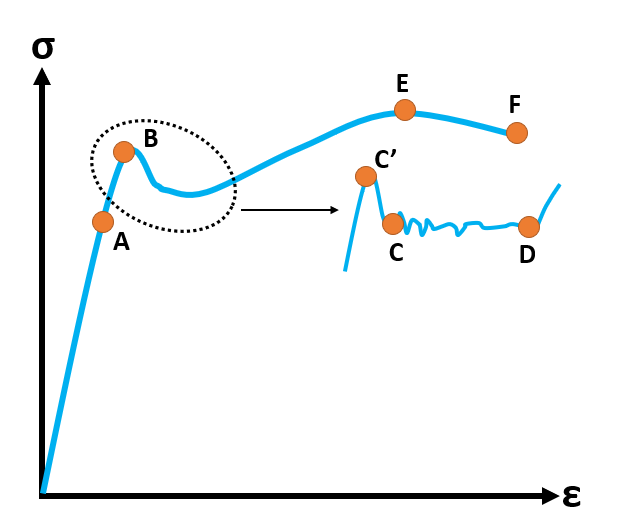
\includegraphics[scale=0.4]{stress-strain-curve.png}
					\centering
				\end{figure}
				\item \underline{\textsc{A = Proportional Limit}}
					\begin{itemize}
						\item \textbf{Hooke's Law: } stress $\propto$ strain
						\item Hooke's law is valid upto this point i.e., Linear variation of stress and strain upto A
					\end{itemize}
				\item \underline{\textsc{B = Elastic limit}}
					\begin{itemize}
						\item Maximum stress upto which material can retain its original dimension upon load removal
						\item Material behaves perfectly elastic up until B
						\item Only Elastic or Elastoplastic deformation (Elastoplastic = both plastic and elastic deformation)
					\end{itemize}
				\item \underline{\textsc{C' = Upper Yield Point}}
					\begin{itemize}
						\item Depends on CS area, shape of specimen and type of the test equipment. 
						\item Has no practical significance
					\end{itemize}
				\item \underline{\textsc{C = Lower Yield Point}}
					\begin{itemize}
						\item Also called as actual yield point and stress at C is the Yield stress($\sigma_y$)
						\item The yielding begins from this point
					\end{itemize}
				\item \underline{\textsc{CD = Perfectly Plastic Region}}
					\begin{itemize}
						\item Strain occurring without any increase in stress
					\end{itemize}
				\item \underline{\textsc{DE = Strain Hardening Region}}
					\begin{itemize}
						\item strain increases with faster rate in this region
						\item material undergoes change in the crystalline structure
					\end{itemize}
				\item \underline{\textsc{E = Ultimate Yield Point}}
					\begin{itemize}
						\item Stress corresponding to this point is called Ultimate stres ($\sigma_U$)
					\end{itemize}
				\item \underline{\textsc{F = Fracture Point}}
					\begin{itemize}
						\item Stress corresponding to this point is called Ultimate  ($\sigma_F$)
						\item Region between EF is called the \textbf{Necking region}, where the CS area is drastically reduced.
					\end{itemize}
			\end{itemize}
		\item \textbf{Plastic Strain:} Strain before Yield point
		\item \textbf{Elastic Strain:} Strain After Yield point
		\item Fracture Strain($\in_F$) depends on Carbon content \%. If carbon($\uparrow$), fracture strain decreases
	\end{itemize}\hrulefill
%-----------------------------------------------------------------------------------------%
\section{Properties of Materials}
	\subsection{Ductility}
		\begin{itemize}
			\item Large deformations are possible in ductile material before fracture
			\item These materials have post-elastic strain greater than 5\%
		\end{itemize}\hrulefill
%-----------------------------------------------------------------------------------------%
	\subsection{Brittleness}
		\begin{itemize}
			\item These materials have post-elastic strain less than 5\%
			\item Fracture takes place immediately after elastic limit
			\item Fracture and ultimate points are the same
		\end{itemize}\hrulefill
%-----------------------------------------------------------------------------------------%
	\subsection{Malleability}
		\begin{itemize}
			\item The property that tells if a metal can be converted into thin sheet by pressing it. 
			\item This property is great use in operations like forging, hot rolling, stamping, etc.,
		\end{itemize}\hrulefill
%-----------------------------------------------------------------------------------------%
	\subsection{Hardness}
		\begin{itemize}
			\item Resistance to scratch or abrasion
			\item Two methods of Hardness measurement:
				\begin{itemize}
					\item Mohr's test
					\item Indentation hardness - Brinell, Rockwell, Vickers, Knoop
				\end{itemize}
		\end{itemize}\hrulefill	%-----------------------------------------------------------------------------------------%
	\subsection{Toughness}
		\begin{itemize}
			\item Property which enables material to absorb energy without fracture.
			\item If a material is tough it has ability to store large amount of strain energy before fracture. 
			\item Ductile materials are tough and brittle materials are hard
			\item \textbf{Modulus of Toughness: }Total strain energy per unit volume up until fracture
			\item Modulus of Toughness = $\boxed{\dfrac{\sigma_y+\sigma_U}{2}*\in_F}$
		\end{itemize}\hrulefill
%-----------------------------------------------------------------------------------------%
	\section{Creep}
		\begin{itemize}
			\item Permanent deformation in a material under constant loading after a long period of time
			\item Factors affecting creep: Load magnitude, type of loading, age of loading, Temperature
			\item \textbf{Homologous temperature: } Half of melting point, creep becomes appreciable at this temperature
		\end{itemize}\hrulefill
%-----------------------------------------------------------------------------------------%
	\section{Stress relaxation}
		\begin{itemize}
			\item The reason why electric wires sag after a long period of time.
			\item The stress gradually diminishes and reaches a constant value after a period of time. 
		\end{itemize}\hrulefill
%-----------------------------------------------------------------------------------------%
	\section{Elasticity}
		\begin{itemize}
			\item The property by which original dimensions can be recovered upon unloading is called elasticity
			\item within elastic limit, the curve can be both linear and non-linear.
		\end{itemize}\hrulefill
%-----------------------------------------------------------------------------------------%
	\section{Resilience}
		\begin{itemize}
			\item The total strain energy which can be stored in the given volume of the metal and can be released after unloading is called resilience.
			\item Resilience = Area under stress-strain curve within elastic limit
			\item \textbf{Modulus of resilience($U_r$): }Maximum elastic energy per unit volume. This occurs when elastic limit coincides with yield point. 
			\item $\boxed{U_r= \dfrac{1}{2}*\sigma_y*\in_y=\dfrac{\sigma_y^2}{2E}}\impliedby \boxed{\in_y=\dfrac{\sigma_y}{E}}$			
	\end{itemize}\hrulefill
%-----------------------------------------------------------------------------------------%
	\section{Proof stress}
		\begin{itemize}
			\item Some materials do not show clear yield point on the stress-strain curve. 
			\item For such materials the yield point is calculated by offset method. 
			\item A line parallel to the curve until the elastic limit is drawn starting from 0.2\% of the strain. This line meets the curve at a point and the corresponding stress at this point is called Proof stress.
		\end{itemize}\hrulefill		%-----------------------------------------------------------------------------------------%
	\section{Elasto-Plastic behaviour}
		\begin{itemize}
			\item during unloading if only part of the original dimension was recovered, then the remaining unrecoverable strain energy is called \textbf{Inelastic strain energy}
			\item Beyond elastic limit, if a material undergoes continuous loading and unloading, then yield limit of material increases continuously
		\end{itemize}\hrulefill
%-----------------------------------------------------------------------------------------%
	\section{Types of Material Behaviour}
		\begin{figure}[H]
			\centering
			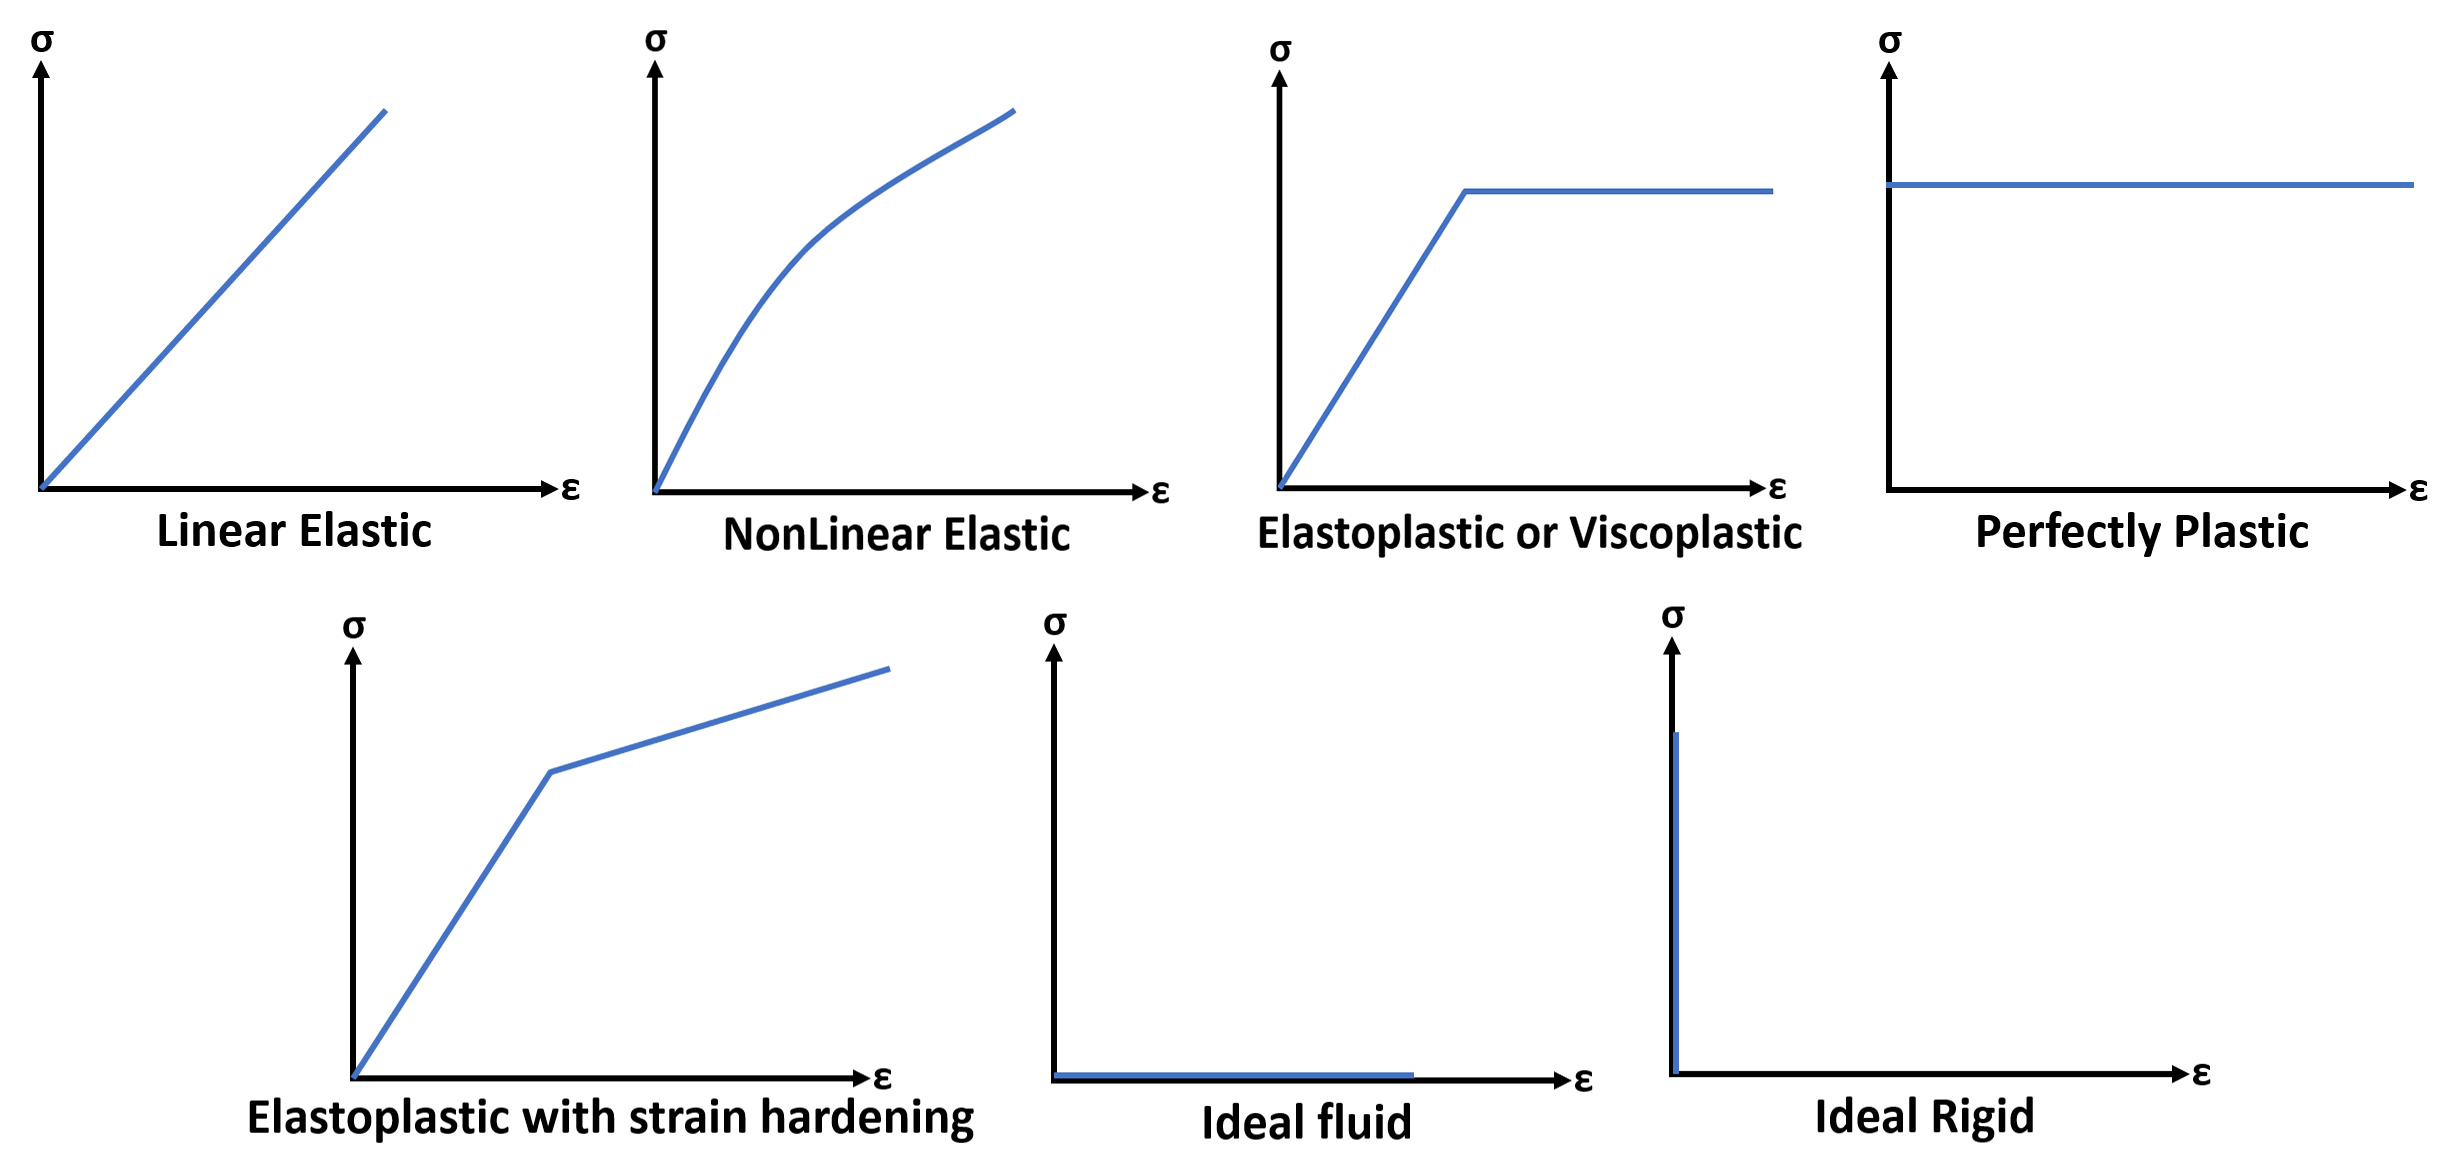
\includegraphics[scale=0.25]{Typesofmaterialbehaviour.png}
		\end{figure}
%-----------------------------------------------------------------------------------------%
	\section{Fatigue}
		\begin{itemize}
			\item Materials behave differently under static and dynamic loading
			\item Factors affecting fatigue: Loading, Temperature, Loading frequency, Corrosion, Stress concentration
			\item \textbf{Fatigue Initiation life: }The number of load cycles required to initiate a surface crack
			\item \textbf{Fatigue Propagation life: }The number additional load cycle required to propagate surface crack
			\item \textbf{Endurance limit: }The stress below which material has no probability of cracking even with infinite load cycles. Endurance limit exists between elastic limit and yield point.
		\end{itemize}\hrulefill
%-----------------------------------------------------------------------------------------%
\section{Failure of Materials in Tension and Compression}
	\subsection{Ductile Metals in Tension}
		\begin{itemize}
			\item Ductile materials are weak in shear
			\item Cup and cone failure
			\item failure plane angle is 45\textdegree
		\end{itemize}\hrulefill
%-----------------------------------------------------------------------------------------%
	\subsection{Brittle Metals in Tension}
		\begin{itemize}
			\item Brittle materials are weak in tension
			\item Failure plane angle is 90\textdegree to load
		\end{itemize}\hrulefill
%-----------------------------------------------------------------------------------------%
	\subsection{Ductile Metals in Compression}
		\begin{itemize}
			\item Failure plane anlge is 90\textdegree to load
		\end{itemize}\hrulefill
%-----------------------------------------------------------------------------------------%
	\subsection{Brittle Metals in Compression}
		\begin{itemize}
			\item Brittle materials fail in shear
			\item Failure plane angle is 45\textdegree
		\end{itemize}\hrulefill
%-----------------------------------------------------------------------------------------%
\chapter{Stress, Strain and Elastic Constants}
	\section{Normal Stress}
		\begin{itemize}
			\item Stress acting perpendicular to the CS area
			\item They are of two types: Direct axial stress, Bending stress
		\end{itemize}
		\subsection{Direct axial stress}
			\begin{itemize}
				\item These stress are produced when axial force is acting at CG of cross section
			\end{itemize}
		\subsection{Bending stress}
			\begin{itemize}
				\item Produced due to Bending moments. Bending stresses vary linearly from 0 at Neutral axis to Maximum at farthest fibre from Neutral Axis
			\end{itemize}\hrulefill
%-----------------------------------------------------------------------------------------%
	\section{Shear (or) Tangential stress($\tau$)}
		\begin{itemize}
			\item Shear stress($\tau$) = $\boxed{\dfrac{ShearForce}{Area} = \dfrac{S}{A}}$
			\item They are of two types: Direct shear, Torsional shear
		\end{itemize}
		\subsection{Direct shear stress}
			\begin{itemize}
				\item Due to direct shear force acting on the surface
			\end{itemize}
		\subsection{Torsional shear stress}
			\begin{itemize}
				\item Produced when a member is subjected to torsional moment (Twisting)
			\end{itemize}\hrulefill
%-----------------------------------------------------------------------------------------%
	\section{Matrix representation of stress and strain}
		\begin{itemize}
			\item Stress and strain are called \textbf{tensor} quantities as are they are defined with respect to an area. They are 2nd order Tensors
			\item In a 3D body, stress or strain at a point has 9 components (3 Normal and 6 shear)
			\item In a 3D, there are 3 mutually perpendicular planes(xy,yz,xz). Each plane has 1 normal component and 2 shear component. 
			\[ \boxed{stress = 
   	 	\left[
        \begin{array}{ccc}
         	\sigma_{xx} & \tau_{xy} & \tau_{xz}\\
         	\tau_{yx} & \sigma_{yy} & \tau_{yz}\\
         	\tau_{zx} & \tau_{zy} & \sigma_{zz}
       	\end{array}
    		\right]}\hspace{2cm}
    		\boxed{
    		strain = 
    		\left[
        \begin{array}{ccc}
         	\in_{xx} & \phi_{xy}/2 & \phi_{xz}/2\\
         	\phi_{yx}/2 & \in_{yy} & \phi_{yz}/2\\
         	\phi_{zx}/2 & \phi_{zy}/2 & \in_{zz}
       	\end{array}
    		\right]}
		\]
			\item Shear stresses in two mutually perpendicular directions are equal: $\tau_{yx} = \tau_{xy}\;\;\tau_{zx}=\tau_{xz}\;\;\tau_{yz}=\tau_{zy}$
			\item Total shear strain in x-y plane: $\dfrac{\phi_{xy}}{2} + \dfrac{\phi_{yx}}{2} = \phi_{xy}$
			\item Total shear strain in y-z plane: $\dfrac{\phi_{zy}}{2} + \dfrac{\phi_{yz}}{2} = \phi_{yz}$
			\item Total shear strain in x-z plane: $\dfrac{\phi_{xz}}{2} + \dfrac{\phi_{zx}}{2} = \phi_{xz}$
			\item $\in_{xx}, \in_{yy}, \in_{zz}$ are linear strains in x, y, z directions respectively
			\item Under pure normal stress = Volume changes, shape remains same
			\item Under pure shear stress = Volume remains same, shape changes.
		\end{itemize}\hrulefill
%-----------------------------------------------------------------------------------------%
		\subsection{Strain Types}
			\subsubsection{Axial Strain($\in$)}
				\begin{itemize}
					\item Strain the direction of the applied force. Also called as \textbf{Linear strain}
					\item $\boxed{\in = \dfrac{Change\;in\;dimension}{original\;dimension} = \dfrac{\Delta L}{L}}$
				\end{itemize}\hrulefill
%-----------------------------------------------------------------------------------------%
			\subsubsection{Lateral Strain($\in_L$)}
				\begin{itemize}
					\item Strain in the direction perpendicular to the applied force. 
					\item Eg. When an object is stretched, its length increases, but its width and height decreases. This decrease in width and height is called Lateral strain. The increase in length is called Linear strain
				\end{itemize}\hrulefill
%-----------------------------------------------------------------------------------------%
			\subsubsection{Shear strain($\phi$)}
				\begin{itemize}
					\item[] 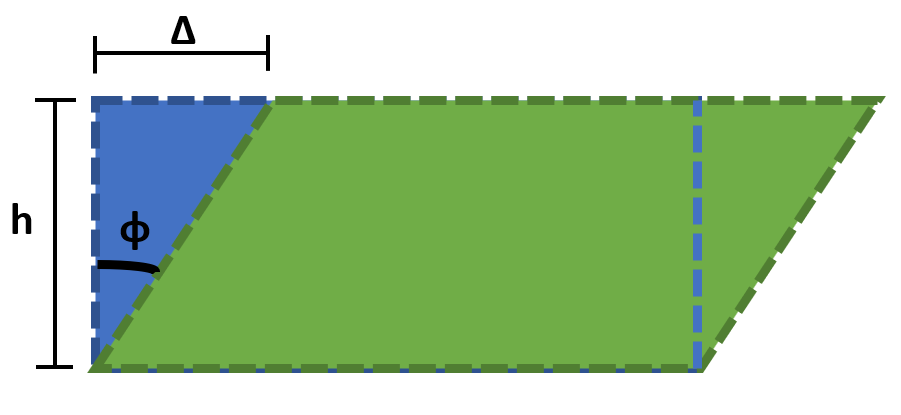
\includegraphics[scale=0.3]{shearstrain.png}
					\item Angular deformation caused by shearing force, $\boxed{\phi = \dfrac{\Delta}{h}}$ 
				\end{itemize}\hrulefill
%-----------------------------------------------------------------------------------------%
		\subsection{Differential form of Strains}
			\begin{itemize}
				\item Consider a point P(x,y,z). A force acting on P, shifts its position to (u,v,w)
				\item Then linear strains and shear strains are given by:
				\item[$\implies$] $\boxed{\in_{xx} = \dfrac{\delta u}{\delta x}}\;\;\; \boxed{\in_{yy} = \dfrac{\delta v}{\delta y}}\;\;\; \boxed{\in_{zz} = \dfrac{\delta w}{\delta z}}\;\;\; \boxed{(\phi_{xy}=\phi_{yx})=\dfrac{\delta u}{\delta y} + \dfrac{\delta v}{\delta x}}\;\;\; \boxed{(\phi_{xz}=\phi_{zx})=\dfrac{\delta w}{\delta x} + \dfrac{\delta u}{\delta z}}\;\;\; \boxed{(\phi_{yz}=\phi_{zy})=\dfrac{\delta w}{\delta y} + \dfrac{\delta v}{\delta z}}\;\;\;$
			\end{itemize}\hrulefill
%-----------------------------------------------------------------------------------------%
	\section{Allowable stresses}
		\begin{itemize}
			\item \textbf{Strength: }The ability of a structure to resist loading is called strength. For safety reasons, materials should have higher strength than what is required due to loading. 
			\item \textbf{Factor of Safety} = $\dfrac{Actual\;strength}{Strength\;required}$
			\item \textbf{Allowable Stress ($\sigma_{A}$)} = $\boxed{\sigma_{A(ductile)}\dfrac{Yield\;stress}{FOS}} = \boxed{\sigma_{A(brittle)}\dfrac{Ultimate\;stress}{FOS}}$
			\item A term called \textbf{Margin of safety} is used for aircrafts. Margin of safety = FOS - 1
		\end{itemize}\hrulefill
%-----------------------------------------------------------------------------------------%
	\section{Saint Venant's principle}
		\begin{itemize}
			\item This principle states that the stress distribution in a prismatic bar is uniform except in the region of extreme ends.
			\item b = width of the prismatic bar
			\item Section(1-1): $\dfrac{b}{2}$ distance from the extreme ends
			\item Section(2-2): $\dfrac{b}{2} + \dfrac{b}{2}$ distance from the extreme ends
			\item $\boxed{\sigma_{1-1}=1.387\sigma_{avg}}\;\;\;\boxed{\sigma_{2-2}=1.027\sigma_{avg}}\;\;\;\boxed{\sigma_{3-3}=\sigma_{avg}}$
		\end{itemize}\hrulefill
%-----------------------------------------------------------------------------------------%
	\section{Hooke's law}
		\begin{itemize}
			\item Assumptions: Homogeneous (made of same material), Isotropic (properties are same in all directions), elastic
			\item Stress $\propto$ Strain $\implies \boxed{\dfrac{\sigma}{\in}=E} \impliedby$ (Valid upto Proportional limit)
			\item E = Modulus of elasticity = slope of stress strain curve under proportional limit 
		\end{itemize}\hrulefill
%-----------------------------------------------------------------------------------------%
	\section{Elastic constants}
		\subsection{Young's modulus(E)}
			\begin{itemize}
				\item $\boxed{E = \dfrac{Direct\;stress}{Direct\;strain} = \dfrac{\sigma}{\in}}$
			\end{itemize}
		\subsection{Shear modulus (or) Rigidity modulus(G)}
			\begin{itemize}
				\item $\boxed{G = \dfrac{Shear\;Stress}{Shear\;strain} = \dfrac{\tau}{\phi}}$
			\end{itemize}
		\subsection{Bulk modulus(k)}
			\begin{itemize}
				\item $\boxed{k = \dfrac{Volumetric\;stress}{Volumetric\;strain} = \dfrac{\sigma_{vol}}{\in_V}}\;\;\;$ $\boxed{\in_V = \dfrac{\Delta Volume}{Volume}}$ 
			\end{itemize}\hrulefill
%-----------------------------------------------------------------------------------------%
		\subsection{Poisson's ratio($\mu$)}
		\begin{itemize}
			\item $\boxed{\mu = \dfrac{-Lateral\;strain}{Linear\;strain}}\impliedby$ (defined in elastic region)
			\item $\mu$ = 0.05 - 1 (glass), 0.1 - 0.2 (concrete),0.25 - 0.42 (metals), 0.5 (pure rubber, perfectly plastic)
			\item For non-elastic region, it is called \textbf{Contraction ratio}
		\end{itemize}\hrulefill
%-----------------------------------------------------------------------------------------%
		\subsection{Relationship between elastic constants}
			\begin{itemize}
				\item $\boxed{E = 3K(1-2\mu)}\;\;\;\boxed{E=2G(1+\mu)}\;\;\;\boxed{E = \dfrac{9KG}{3K+G}}\;\;\;\boxed{\mu = \dfrac{3K-2G}{6K+2G}}$
				\item \textbf{Orthotropic material} = 9 elastic constants, \textbf{Anisotropic material} = 21 elastic constants
			\end{itemize}\hrulefill
%-----------------------------------------------------------------------------------------%
	\section{Applications of Hooke's law}
		\subsection{Effect of Uniaxial Loading}
			\begin{itemize}
				\item Consider a rectangular prismatic bar with tensile force acting along x-axis
				\item[] $\boxed{\in_{xx} = \dfrac{\sigma_x}{E}} \implies \boxed{\in_{yy} = -\mu\dfrac{\sigma_x}{E}}\;\boxed{\in_{zz}=-\mu\dfrac{\sigma_x}{E}} \impliedby \in_{yy}\;\&\;\in_{zz}$ are Lateral strains
			\end{itemize}
		\subsection{Effect of Triaxial Loading}
			\begin{itemize}
				\item Consider: $\sigma_x$ acting along x-direction, $\sigma_y$ acting along x-direction, $\sigma_z$ acting along x-direction. (All are Tensile)
				\item $\boxed{\in_{xx} = \dfrac{\sigma_x}{E} -\mu\dfrac{\sigma_y}{E} -\mu\dfrac{\sigma_z}{E}}\;\;\;$ $\boxed{\in_{yy} = \dfrac{\sigma_y}{E} -\mu\dfrac{\sigma_x}{E} -\mu\dfrac{\sigma_z}{E}}\;\;\;$ $\boxed{\in_{zz} = \dfrac{\sigma_z}{E} -\mu\dfrac{\sigma_x}{E} -\mu\dfrac{\sigma_y}{E}}$
			\end{itemize}\hrulefill	%-----------------------------------------------------------------------------------------%
	\section{Volumetric Strain($\in_V$)}
		\begin{itemize}
			\item How to derive?
			\item compute the volume of the member. take that as V.
			\item Now find $\Delta V$, that is differentiate V wrt to each factor.
			\item Then use: $\boxed{\in_V = \in_x+\in_y+\in_z}$
		\end{itemize}
		\subsection{For Rectangular prismatic member}
			\begin{itemize}
				\item $\boxed{\dfrac{\sigma_x+\sigma_y+\sigma_z}{E}*(1-2\mu)}$
			\end{itemize}
		\subsection{For Cylindrical rod}
			\begin{itemize}
				\item $\boxed{\in_V=\in_L+2\in_d} \impliedby (\in_d$ = Diametrical strain)
			\end{itemize}
		\subsection{For Spherical body}
			\begin{itemize}
				\item $\boxed{\in_V=3\in_d}$
			\end{itemize}\hrulefill
%-----------------------------------------------------------------------------------------%
	\section{Elongation in axially loaded members}
		\begin{itemize}
			\item How to derive?
			\item consider an element and find its elongation using $\dfrac{PL}{AE}$, Then integrate that $\delta L$ for the whole length
		\end{itemize}
		\subsection{Axially loaded prismatic bar}
			\begin{itemize}
				\item In this case Elemental elongation is $\dfrac{P_xd_x}{A_xE_x} \impliedby d_x$ = Length of the element. 
				\item $\boxed{\Delta = \dfrac{PL}{AE}}\;\;\;\;$ ($AE$ = Axial rigidity) and ($\dfrac{AE}{L}$ = Axial stiffness)
			\end{itemize}
		\subsection{Axially loaded Circular Tapered bar}
			\begin{itemize}
				\item Here Diamater of the element = $D_x = D_1+\dfrac{D_2-D_1}{L}x$
				\item $\boxed{\Delta = \dfrac{4PL}{\pi E D_1D_2}} \impliedby D_1 =$ smaller diameter and $D_2$ = Larger diameter
			\end{itemize}
		\subsection{Axially loaded Rectangular Tapered bar}
			\begin{itemize}
				\item The thickness of the bar is uniform
				\item $\boxed{\Delta = \dfrac{PL\log_e\left(\dfrac{B_2}{B_1}\right)}{(B_2-B_1)tE}} \impliedby$ ($B_1$ = Smaller height and $B_2$ = Larger height)
			\end{itemize}\hrulefill
%-----------------------------------------------------------------------------------------%
	\section{Principle of Superposition}
		\begin{itemize}
			\item If a member is subjected to various loadings then the resultant deformation will be equal to the algebraic sum of the deformation caused by the individual forces acting on the member.
			\item Consider the following example:
			\begin{figure}[H]
				\centering
				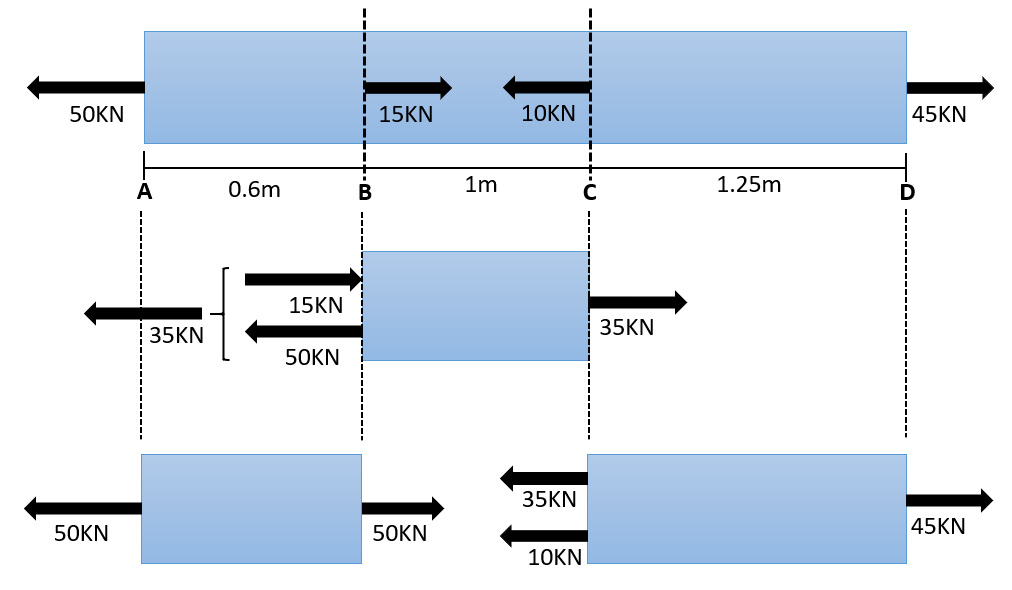
\includegraphics[scale=0.5]{superposition.png}
			\end{figure}
			\item Total elongation of the element($\Delta$) = $\Delta_{AB}+\Delta_{BC}+\Delta_{CD}$
		\end{itemize}\hrulefill
%-----------------------------------------------------------------------------------------%
	\section{Elongation in Composite members}
		\begin{itemize}
			\item Composite structures are those that are made of more than one material
		\end{itemize}
		\subsection{Elongation in composite rectangular member}
			\begin{itemize}
				\begin{figure}[H]
					\centering
					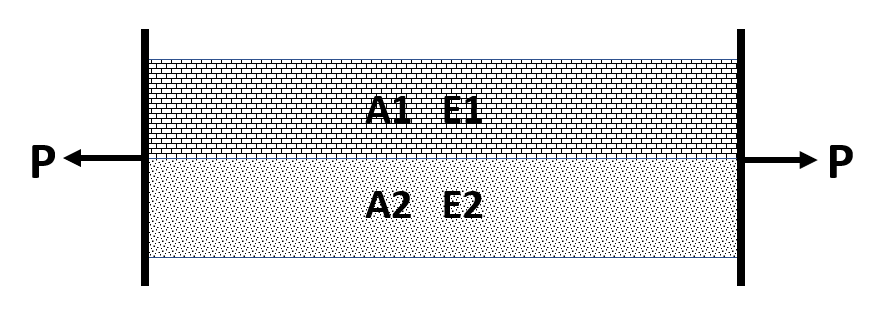
\includegraphics[scale=0.5]{compositebar.png}
				\end{figure}
				\item Condition of Equilibrium: $P = P_1+P_2$
				\item As two materials are joined firmly: $\Delta_1 = \Delta_2 \implies \dfrac{P_1L_1}{A_1E_1} = \dfrac{P_2L_2}{A_2E_2}$
				\item $\boxed{\Delta = \dfrac{PL}{A_1E_1+A_2E_2}}$ and $E_{eq} = \dfrac{A_1E_1+A_2E_2}{A_1+A_2} \implies \Delta = \dfrac{PL}{(A_1+A_2)E_{eq}}$
			\end{itemize}\hrulefill
%-----------------------------------------------------------------------------------------%
	\section{Elongation due to Self-Weight}
		\begin{itemize}
			\item How to derive?
			\item Find the elemental deflection due to the self weight and then Integrate for the whole length. 
		\end{itemize}
		\subsection{Rectangular Prismatic bar}		
			\begin{itemize}
				\item $\gamma = Unit\;weight = \dfrac{Weight}{unit\;volume}$
				\item $W_x = \gamma (A*x) \impliedby W_x$ = Self weight acting at an element x distance away from the bottom of the bar				
				\item $\boxed{\Delta = \dfrac{\gamma L^2}{2E}} \implies \boxed{\dfrac{WL}{2AE}}$
			\end{itemize}
		\subsection{Conical Bar}
			\begin{itemize}
				\item $\boxed{W_x = \gamma*\left(\dfrac{1}{3}\right)\pi\left(\dfrac{D_x}{2}\right)^2x}$ $\;\;\;\boxed{\Delta = \dfrac{\gamma L^2}{6E}}$
			\end{itemize}
		\subsection{Bar of Uniform strength}
			\begin{itemize}
				\item It is possible to maintain uniform stress at all the sections by increasing the area from the lower level to Higher level.
				\item $\boxed{A_1=A_2e^{\left(\dfrac{\rho gL}{\sigma}\right)}}$
			\end{itemize}\hrulefill
%-----------------------------------------------------------------------------------------%
	\section{Statically Indeterminate Axial Loaded structures}
		\begin{itemize}
			\item Those structures which cannot be solved using static equilibrium equations alone are called Statically Indeterminate structures
			\item They can be solved using flexibility approach or stiffness approach
			\item Flexibility approach involves equations using the relations in Slope, deflection and rotation and are called \textbf{compatibility equation}
		\end{itemize}\hrulefill
%-----------------------------------------------------------------------------------------%
	\section{Thermal stresses}
		\begin{itemize}
			\item \textbf{NOTE: }Thermal stresses do not depend on the area of cross section
			\item Thermal Strain $\boxed{\in_{Th} = \alpha T} \impliedby (\alpha$ = Coefficient of thermal expansion)
			\item Consider a rectangular prismatic bar of length L between fixed supports. If the temperature of the bar is raised, then $\Delta = 0$ (As the bar is fixed)
			\item But due to rise in temperature of T\textdegree C, the bar will try to expand and so will be under compression
			\item $\Delta = 0 = L\alpha T - \dfrac{\sigma_{Th} L}{E} \implies \boxed{\sigma_{Th} = E\alpha T} \impliedby$ (Thermal stresses are independent of member dimensions)
		\end{itemize}\hrulefill
%-----------------------------------------------------------------------------------------%
		\subsection{Thermal stresses in Composite bars}
			\begin{itemize}
				\item Mostly we use three sets of relations 
				\item $P_1 = P_2$ (under no other external load) $\implies \sigma_1A_1 = \sigma_2A_2$
				\item $\Delta_1 = \Delta_2$
				\item The material with larger $\alpha$ value, will tend to deform more under thermal load
				\item Consider a composite cantilever bar made of copper and steel and both the materials are rigidly fixed to each other. Copper has higher coefficient of thermal expansion and so upon temperature rise will tend to expand more than steel. 
				\item As a result, copper part will be under compression as steel is not letting it to expand and steel part will be under tension as copper is pulling it.
				\item As they are affixed to each other rigidly, both their end deformation value will be the same. Using that relation we can write: Copper free expansion + contraction = steel free expansion + tension  $\implies \boxed{L\alpha_cT-\dfrac{\sigma_cL}{E_c}=L\alpha_sT+\dfrac{\sigma_sL}{E_s}}$
			\end{itemize}\hrulefill
%-----------------------------------------------------------------------------------------%
	\section{Stresses in Nuts and Bolts}
		\begin{itemize}
			\item \textbf{Effect of Tightening of Nut}
			\item P = pitch of screw on the bolt, $D_b$ = Bolt diameter
			\item $A_s$ = Area of steel bolt = $\dfrac{\pi D_b^2}{4}$
			\item $D_i$ = Inner diameter of copper tube, $D_O$ = Outer diameter of copper tube
			\item $\theta$ = Nut is rotated by $\theta$\textdegree, n = Number of turns = $\dfrac{\theta}{360}$
			\item np = Axial movement of nut
			\item Total tensile for in bolt = total compressive force in copper tube $\implies \sigma_sA_s = \sigma_cA_c$
			\item $\boxed{np = \left(\dfrac{\sigma_sL}{E_s}\right)+\left(\dfrac{\sigma_cL}{E_c}\right)}\impliedby$ Using the above relation, solve for $\sigma_s$ and $\sigma_c$
		\end{itemize}\hrulefill
%-----------------------------------------------------------------------------------------%
	\section{Strain Energy(U)}
		\begin{itemize}
			\item The strain energy is equal to the work done by the load provided no energy is added or subtracted in the form of heat.
			\item \textbf{NOTE: } Strain energy due to more than one load can be found by applying Superposition principle. i.e. Total strain energy due to multiple loads = Sum of individual strain energy developed due to individual loads
			\item $\boxed{U = \dfrac{1}{2}P\Delta} \impliedby \Delta$ = Axial deflection 
		\end{itemize}\hrulefill
		\subsection{Strain energy in Prismatic bar}
			\begin{itemize}
				\item $\boxed{U = \dfrac{P^2L}{2AE}}$
			\end{itemize}\hrulefill
		\subsection{Strain energy in Prismatic bar of varying cross section}
			\begin{itemize}
				\item $\boxed{U = \dfrac{P^2}{2E}\left[\dfrac{L_1}{A_1}+\dfrac{L_2}{A_2}+...\right]}$
			\end{itemize}\hrulefill
		\subsection{Strain energy due to shear force}
			\begin{itemize}
				\item $\boxed{U = \int\dfrac{S_x^2dx}{2A_rG}}\implies (A_r$ = Reduced area)
			\end{itemize}\hrulefill
		\subsection{Strain energy in terms of principal stresses}
			\begin{itemize}
				\item $\boxed{U = \dfrac{1}{2E}(\sigma_1^2+\sigma_2^2-2\mu\sigma_1\sigma_2)} \impliedby$ (2D) $\;\;\;\boxed{U = \dfrac{1}{2E}\left[\sigma_1^2+\sigma_2^2+\sigma_3^2-2\mu(\sigma_1\sigma_2+\sigma_2\sigma_3+\sigma_3\sigma_1)\right]} \impliedby$ (3D)
			\end{itemize}\hrulefill
		\subsection{Strain energy due to Bending moment}
			\begin{itemize}
				\item $\boxed{U = \int\dfrac{M_x^2ds}{2EI}}\impliedby$ (I = MOI about NA)
			\end{itemize}\hrulefill
		\subsection{Strain energy due to Torque}
			\begin{itemize}
				\item $\boxed{U = \int\dfrac{T_x^2ds}{2GI_P}}\impliedby (I_P$ = Polar MOI)
			\end{itemize}\hrulefill
%-----------------------------------------------------------------------------------------%
\chapter{Shear force and Bending Moment}
	\section{Types of Loading}
		\begin{itemize}
			\item Point load
			\item Uniformly Distributed Load
			\item Uniformly Varying Load
			\item Couple - Concentrated moment at any point is called couple
		\end{itemize}\hrulefill
%-----------------------------------------------------------------------------------------%
	\section{Types of supports}	
		\subsection{Types of 2D Supports}
			\begin{itemize}
				\item Fixed support - $R_x,R_y,M_z$
				\item Hinged Support - $R_x,R_y$
				\item Roller support - $R_y$
				\item Double roller support - $R_y,M_z$
			\end{itemize}
		\subsection{Types of 3D Supports}
			\begin{itemize}
				\item Fixed support - $R_x,R_y,R_z,M_x,M_y.M_z$
				\item Hinged support - $R_x,R_y,R_z$
				\item Roller support - $R$
			\end{itemize}\hrulefill			
%-----------------------------------------------------------------------------------------%
	\section{Types of Beams}
		\begin{itemize}
			\item Simply supported beam
			\item Cantilever beam
			\item Propped cantilever beam
			\item Fixed beam
			\item Continuous beam
			\item Overhanging beam
			\item \textbf{NOTE: If an internal hinge is present in a beam, then Bending moment at hinge is Zero. Hinges carry only Axial load.}
		\end{itemize}\hrulefill
%-----------------------------------------------------------------------------------------%
	\section{Statically determinate structure}
		\begin{itemize}
			\item A structure is said to be statically determinate if all the reaction forces can be found using the static equilibrium equations (2D): $\boxed{\sum F_x=0\;\;\sum F_y=0\;\;\sum M_z=0}$
			\item If R denotes the number of reactions and E denotes the number of equilibrium equations available, then if (R $=$ E ) the structure is determinate, if (R $>$ E) then the structure is indeterminate
		\end{itemize}\hrulefill
%-----------------------------------------------------------------------------------------%
	\section{Shear Force}
		\begin{itemize}
			\item Clockwise shear = +ve and Anticlockwise shear = -ve
		\end{itemize}\hrulefill
%-----------------------------------------------------------------------------------------%
	\section{Bending Moment}
		\begin{itemize}
			\item Sagging Bending moment = +ve and Hogging Bending moment = -ve
		\end{itemize}\hrulefill
%-----------------------------------------------------------------------------------------%
	\section{Important points about SFD and BMD}
		\begin{itemize}
			\item SFD is one degree higher than Loading diagram and BMD is one degree higher than SFD
			\item If a point load is present, then the SFD will change by that load's magnitude
			\item If a concentrated moment is present, then the BMD will change by that moment's magnitude
			\item Bending will be maximum/minimum at the point where Shear force is zero, but the inverse is not true
			\item \textbf{Point of Contraflexure} - The point where Bending moment changes sign
			\item \textbf{Focal length} - The distance between two adjacent points of contraflexure
			\item \textbf{Shear span} - the portion of beam where shear force is constant.
			\item Relation between Loading rate and Shear force: $\boxed{\dfrac{dS}{dx}=-W}$
			\item Relation between Shear force and bending moment: $\boxed{\dfrac{dM}{dx}=S_x}\implies$ Slope of bending moment = shear force.
			\item Relation between Bending moment and Loading rate: $\boxed{\dfrac{d^2M}{dx^2}=-w}$
		\end{itemize}\hrulefill
%-----------------------------------------------------------------------------------------%
	\section{Curve Tracing for SFD and BMD}
			\begin{figure}[H]
				\centering
				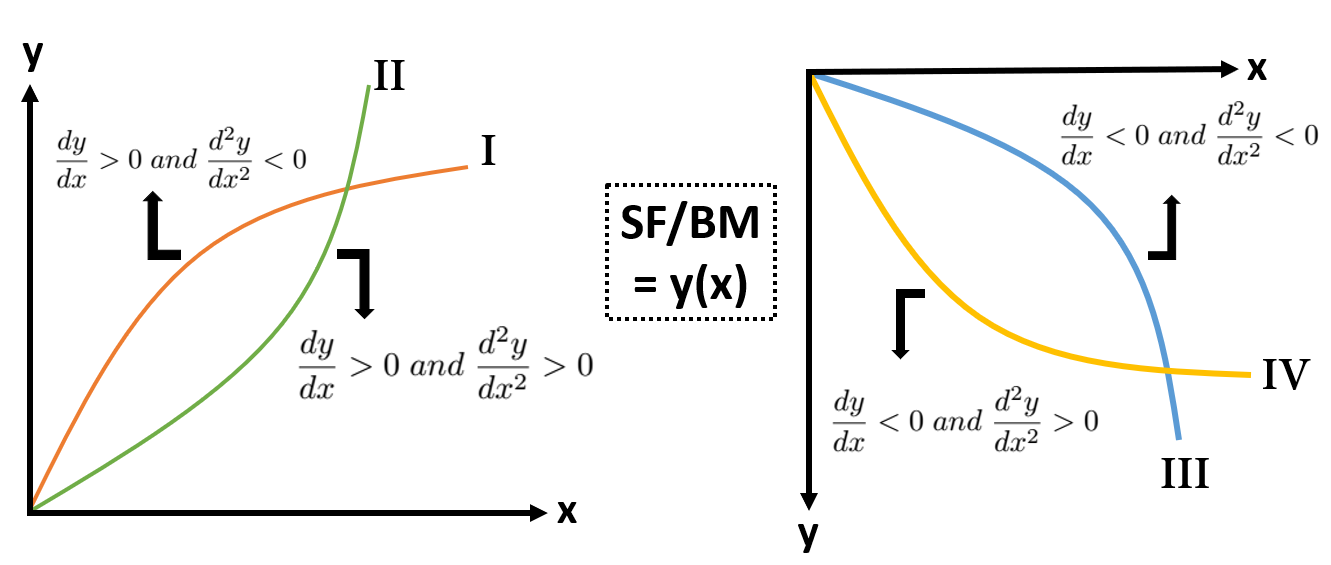
\includegraphics[scale=0.4]{curvetracing.png}
			\end{figure}\hrulefill
%-----------------------------------------------------------------------------------------%
	\section{SFD and BMD by Integration}
		\begin{itemize}
			\item Use the relations between Loading rate, shear force and Bending moment:
				\begin{itemize}
					\item[$\implies$] $\boxed{\dfrac{d^2M}{dx^2}=-w}\;\;\;$...(i)  $\boxed{\dfrac{dM}{dx}=S_x=-Wx+C_1}\;\;\;$...(ii)  $\boxed{M_x = \dfrac{-Wx^2}{2} + C_1x + C_2}$   ...(iii)
					\item \textbf{NOTE: } Eqn(i)'s RHS will change according the loading. For eg. in case of Uniformly variying load, $$\boxed{\dfrac{d^2M}{dx^2}= -W_x = \dfrac{-Wx}{L}}$$
				\end{itemize}
			\item The constants $C_1$ and $C_2$ can be found by boundary conditions
			\item From (ii) SFD can be plotted, from (iii) BMD can be plotted
		\end{itemize}\hrulefill
%-----------------------------------------------------------------------------------------%
	\section{Effect of Concentrated moment on SFD and BMD}
		\begin{itemize}
			\item At the point of concentrated moment, discontinuity occurs in BMD. The BMD ordinate changes by the magnitude of the moment. For SFD, concentrated moment induces support reactions only.
			\begin{figure}[H]
				\centering
				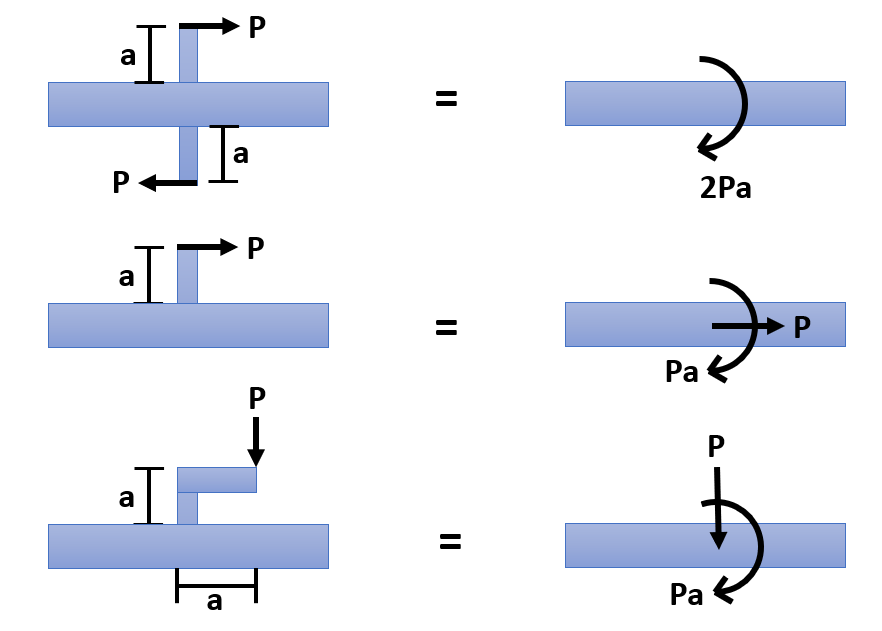
\includegraphics[scale=0.5]{concmoment}
			\end{figure}
		\end{itemize}\hrulefill
%-----------------------------------------------------------------------------------------%
	\section{Loading diagram and BMD from SFD}
		\begin{itemize}
			\item In SFD, the portion where SF is constant, it means no load is acting in that portion
			\item In SFD, Vertical lines represent loads (Generally upward loads denote reactions)
			\item Inclined line in SFD denotes Uniformly distributed load. Intensity of UDL = slope of line in SFD
			\item Parabolic curve in SFD denotes Uniformly varying load. 
			\item If $\sum M$ at supports is zero, then the support is hinged or roller. If its not zero, then it is a fixed support.
	\end{itemize}\hrulefill
%-----------------------------------------------------------------------------------------%
	\section{Loading diagram from BMD}
		\begin{itemize}
			\item In BMD, the portion where there is an inclined line, that means no load is acting in that region
			\item Parabolic curve in BMD denotes Unifromly distributed load. 
			\item Cubic curve in BMD denotes Uniformly varying load.
			\item The point where BMD changes its ordinate suddenly, a concentrated moment is acting at that point. 
			\item BMD is one degree higher than SFD and two degree higher than Loading diagram
		\end{itemize}\hrulefill
%-----------------------------------------------------------------------------------------%
\chapter{Centroid and Moment of Inertia}
	\section{Centroid($\bm{\bar{x}}$,$\bm{\bar{y}}$)}
		\begin{itemize}
			\item $\boxed{\bar{x} = \dfrac{A_1\bar{x_1}+A_2\bar{x_2}+...+A_n\bar{x_n}}{A_1+A_2+...+A_n} = \sum_{i=1}^{n}\dfrac{A_i\bar{x_i}}{A_i} =\dfrac{\int xdA}{A}}\;\;\;\boxed{\bar{y}=\dfrac{A_1\bar{y_1}+A_2\bar{y_2}+...+A_n\bar{y_n}}{A_1+A_2+...+A_n} = \sum_{i=1}^{n}\dfrac{A_i\bar{y_i}}{A_i} =\dfrac{\int ydA}{A}}$
			\item It is the center of a shape
				\begin{itemize}
					\item If the shape is Bi-Symmetrical, then the centroid will lie on the point of intersection of the two symmetrical axis. Eg. Rectangle, Square, Circle, etc.
					\item If the shape is symmetrical about only one axis, then centroid will be anywhere on that symmetrical axis. Eg. Triangle
				\end{itemize}
		\end{itemize}\hrulefill
%-----------------------------------------------------------------------------------------%
	\subsection{Finding centroid for a composite shape}
		\begin{itemize}
			\item A composite shape is a shape that is made of many regular shapes like: semicircle, circle, rectangle, square etc,
			\item How to find Centroid for a composite shape? An example of composite shape is shown below
			\begin{figure}[H]
				\centering
				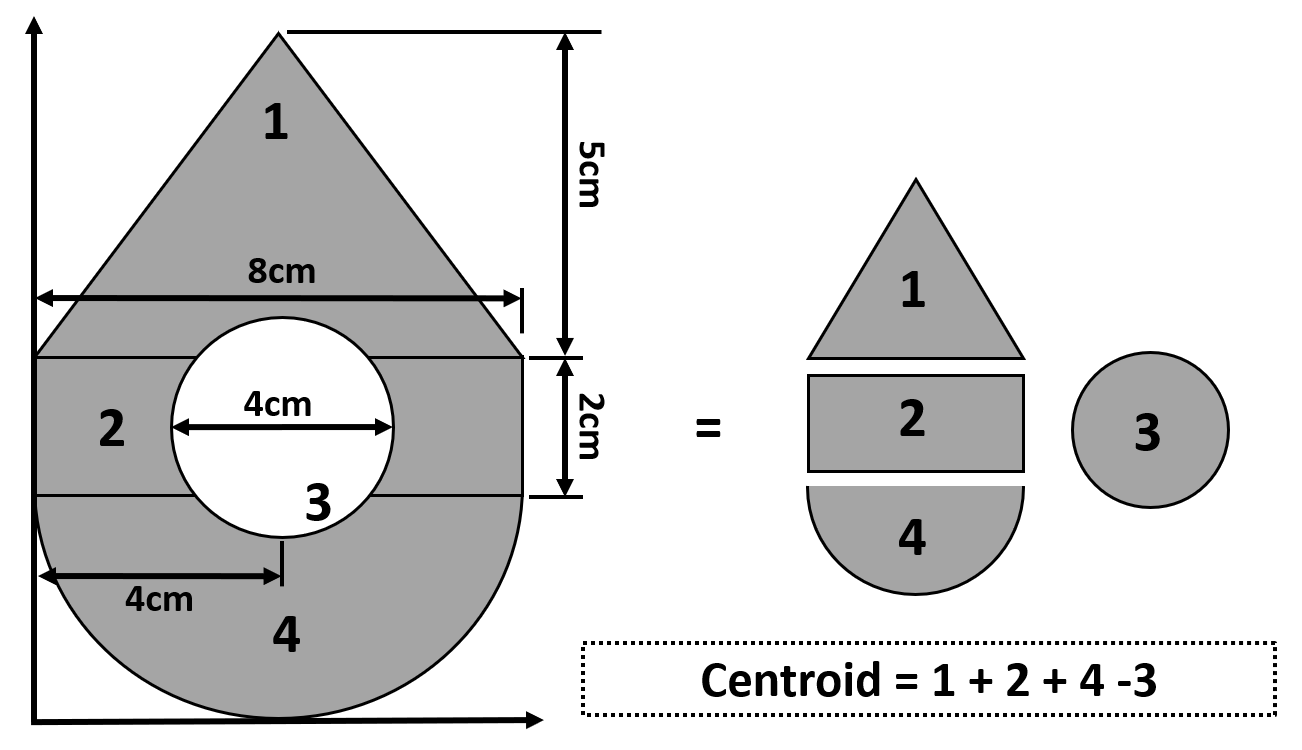
\includegraphics[scale=0.4]{breakingcomposite.png}\\
			\end{figure}
			\item Break down the composite shapes into its regular shapes. Then form a table with the following columns: $$shape,\;\;Area(A),\;\;\bar{x},\;\;\bar{y},\;\;A\bar{x},\;\;A\bar{y}$$ 
			\item Then find: $\sum A$, $\sum A\bar{x}$, $\sum A\bar{y}$ and then use, $\bar{x} = \dfrac{\sum A\bar{x}}{\sum A}$ and $\bar{y} = \dfrac{\sum A\bar{y}}{\sum A}$
			\item For example, the above shape can be broken down into 4 parts as shown above: Triangle, Rectangle, Circle and Semi-circle
			\item Now, we need to know 3 things about each of the shape above to compute the centroid of the whole shape. 
				\begin{enumerate}
					\item Area of the shape\hspace{1cm}$2.\;\bar{x}$\hspace{1cm}$3.\;\bar{y}$				
				\end{enumerate}
			\item For triangle: 
				\begin{itemize}
					\item[$\rightarrow$] Area:$\;\;\left(\dfrac{1}{2}*Base*Height\right) = \dfrac{1}{2}*8*5 = 20cm^2$
					\item[$\rightarrow$] $\bar{x}$ = Base/2 (as the triangle is symmetrical about the y-axis) = 4cm
					\item[$\rightarrow$] $\bar{y}$ = 10 + h/3 = (10+1.6667cm)
						\begin{itemize}
							\item 10 is added because, the triangle is at a height of 10cm from x-axis
							\item Why $\bar{y}$ = h/3 ? Derived below:
						\end{itemize}
				\end{itemize}							
		\end{itemize}\hrulefill
%-----------------------------------------------------------------------------------------%
	\subsection{Finding $\bar{y}$ for a triangle}
		\begin{itemize}
			\begin{figure}[H]
				\centering
				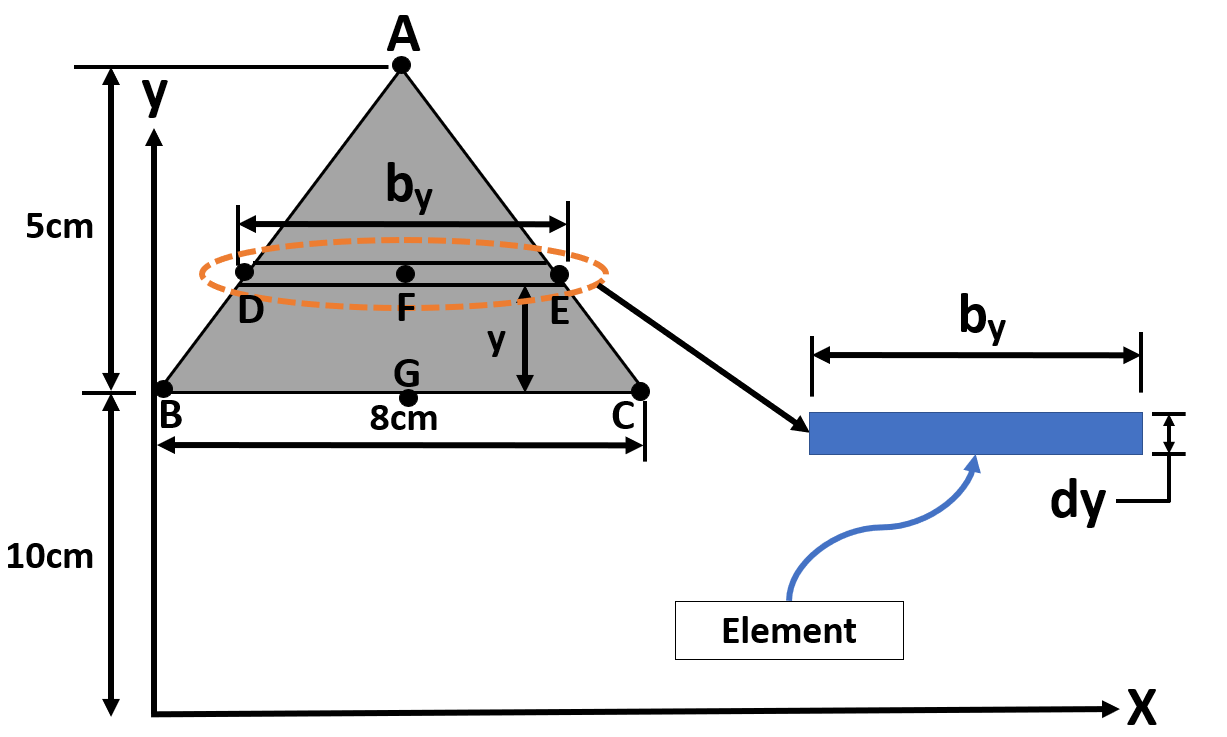
\includegraphics[scale=0.5]{triangleybar.png}
			\end{figure}
			\item We know that $\boxed{\bar{y}=\dfrac{A_1\bar{y_1}+A_2\bar{y_2}+...+A_n\bar{y_n}}{A_1+A_2+...+A_n} = \sum_{i=1}^{n}\dfrac{A_i\bar{y_i}}{A_i} = \dfrac{\sum A_i\bar{y_i}}{A}}$
			\item Here, Area = 20$cm^2$
			\item Consider a horizontal element of thickness (dy) at a height of y from origin. 
			\item The width of the element can be found using \textbf{Law of similar triangles} concept. Based on that: $$\dfrac{AG}{BC}=\dfrac{AF}{DE}\implies\dfrac{5}{8}=\dfrac{5-y}{b_y}\implies b_y = \dfrac{8(5-y)}{5}$$
			\item Now, Area of this element is $A_i = b_ydy = \dfrac{8(5-y)}{5}dy$ and $\bar{y}_i = 10+y+\dfrac{dy}{2} \impliedby$ But already dy is very small. So dy/2 is negligble $\implies\bar{y}_i=10+y$ 
			\item Applying the formula of $\bar{y}$ we get, 
			\begin{align*}
				\bar{y} &= \dfrac{\sum \dfrac{8(5-y)}{5}dy(10+y)}{20}\;\;=\;\; \dfrac{\bigintss_0^5\dfrac{8(5-y)}{5}(10+y)dy}{20}\\
				&= \dfrac{1}{100}\int_0^5(40-8y)(10+y)dy\;\;=\;\;\dfrac{1}{100}\int_0^5 400+40y-80y-8y^2\;\;=\;\;\dfrac{1}{100}\int_0^5 400-40y-8y^2\\
				&= \dfrac{8}{100}\int_0^5 50-5y-y^2\;\;=\;\;0.08*\left[50y-5\dfrac{y^2}{2}-\dfrac{y^3}{3}\right]_0^5\;\;=\;\;0.08*\left[50(5)-5(12.5)-\dfrac{125}{3}\right]\\
				&= 0.08 * (145.833) = 11.667 \implies 10 + 1.667 \implies 10 + 5/3 \implies 10+h/3
			\end{align*}						
			\item Hence, $\bar{y}$ for a triangle is h/3
		\end{itemize}\hrulefill
%-----------------------------------------------------------------------------------------%
	\subsection{Finding centroid for area under a given curve}
		\begin{itemize}
			\item Consider a vertical strip of thickness(dx) at a distance of x from origin and height(y)=f(x)
			\item The area of this element will be dA = ydx = f(x)dx
			\item Integrate this small area over the entire width of the curve and find Total area(A).
			\item Use the formula, $\bar{x} = \dfrac{\int xdA}{A}$ and $\bar{y}=\dfrac{\int ydA}{A}$
		\end{itemize}\hrulefill
%-----------------------------------------------------------------------------------------%
	\section{Moment of Inertia (I)}
		\begin{itemize}
			\item Normally Inertia means, from Newton's first law, it is the resistance to change  of state.
			\item Moment of Inertia are of various types.
				\begin{itemize}
					\item Area Moment of Inertia -  Resistance to Bending
					\item Mass Moment of Inertia - Resistance to Rotation (based on mass distribution)
					\item Polar Moment of Inertia - Resistance to Twisting (based on Perpendicular axis theorem)
					\item Product of Inertia - Resistance to Rotation (based on two perpendicular axes)
				\end{itemize}
			\item Here we are concerned with Area MOI and Polar MOI
			\item Area MOI is also called as 2nd moment of Area. 
			\item Area MOI is always Non-zero and Positive
			\item Area MOI about x-axis = $\boxed{I_{x} = \int y^2dA}\;\;\;$ Area MOI about y-axis = $\boxed{I_{y} = \int x^2dA}$
			\item The further a material is spread from its bending axis, the more resistant it is towards bending. See the figure below for better understanding.
			\item The Area MOI of a section is lowest if it is taken about an axis passing through the centroid of the section
			\begin{figure}[H]
				\centering
				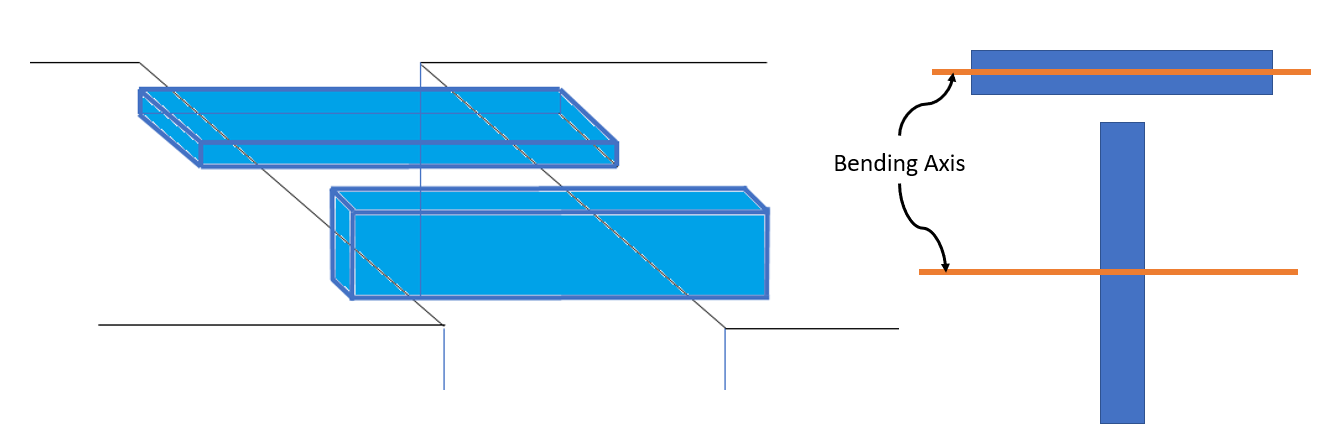
\includegraphics[scale=0.4]{bending.png}
			\end{figure}
			\item In the figure above, the first bar is flatly laid. When a load is acting at its center, its more prone to bending and hence breaking compared to the same bar that is laid in a different position and subjected to the same load. 
			\item Because, in the first bar, the material is less spread from the bending axis, compared to the second bar
			\item This demonstrates why computing MOI is very important to consider the safety of structures. 
		\end{itemize}\hrulefill
%-----------------------------------------------------------------------------------------%
	\subsection{Steps to find Area MOI for any area}
		\begin{itemize}
			\item Consider elementary strip (horizontal strip for $I_x$ and vertical strip for $I_y$) and find it's area (dA)
			\item Use the above two formula with appropriate limits
		\end{itemize}
	\subsection{Finding Area MOI for a rectangle about its centroidal axis}
		\begin{itemize}
			\item Remember: $(\;\int_{-a}^a(even\;function) = 2\int_0^a(even\;function))$
			\begin{figure}[H]
				\centering
				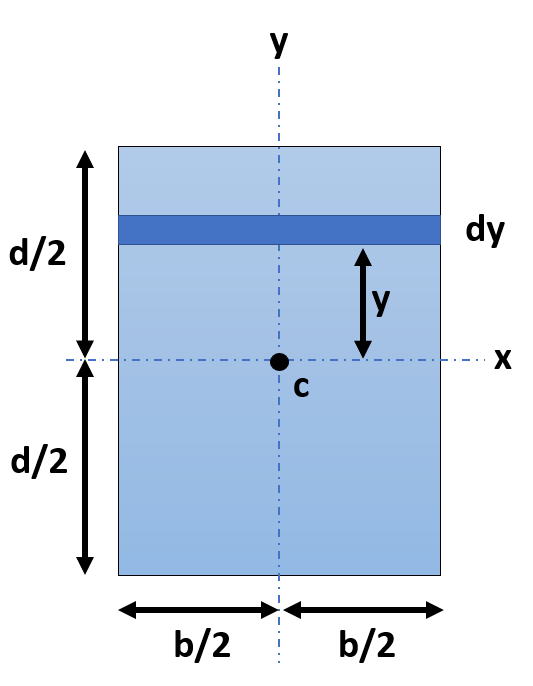
\includegraphics[scale=0.35]{rectangleMOI_Ix.png}\hspace{3cm}
				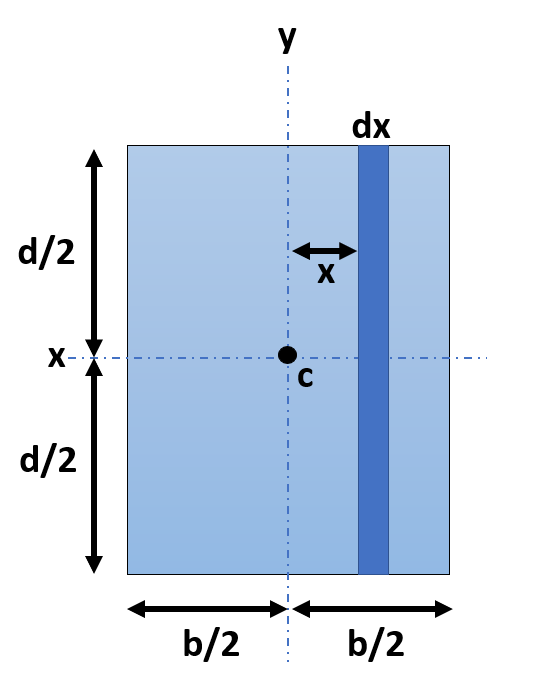
\includegraphics[scale=0.35]{rectangleMOI_Iy.png}
			\end{figure}
		\end{itemize}
			\begin{table}[H]
				\centering
				\begin{tabular}{c|c}
					{$\begin{aligned}
					dA&=b(dy)\\
					We\;know\;I_x &= \int y^2dA\\
					I_x &= \int_{-d/2}^{d/2}y^2(bdy) = 2b\int_0^{d/2}y^2dy\\
					I_x &= 2b\left(\dfrac{y^3}{3}\right)_0^{d/2} = 2b\left(\dfrac{d^3}{8*3}\right)\\
					\Aboxed{I_x &= \dfrac{bd^3}{12}}
					\end{aligned}$}&
					
					{$\begin{aligned}
					dA &= d(dx)\\
					We\;know\;I_y &= \int x^2dA\\
					I_y &= \int_{-b/2}^{b/2}x^2(d(dx)) = 2d\int_{0}^{b/2}x^2dx \\
					I_y &= 2d\left(\dfrac{x^3}{3}\right)_0^{b/2} = 2d\left(\dfrac{b^3}{8*3}\right)\\
					\Aboxed{I_y &= \dfrac{db^3}{12}}
					\end{aligned}$}
				\end{tabular}
			\end{table}\hrulefill
%-----------------------------------------------------------------------------------------%
	\subsection{Finding Area MOI for a rectangle with origin at bottom left corner}
		\begin{figure}[H]
				\centering
				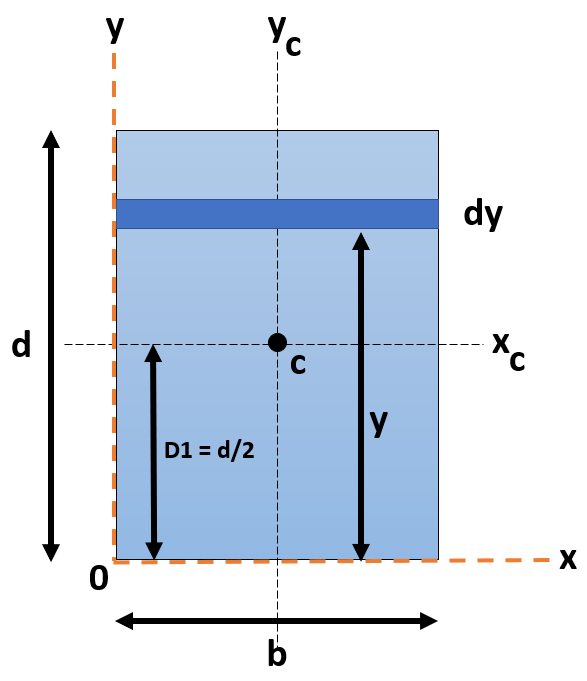
\includegraphics[scale=0.4]{rectangleMOIcorner_Ix.png}\hspace{3cm}
				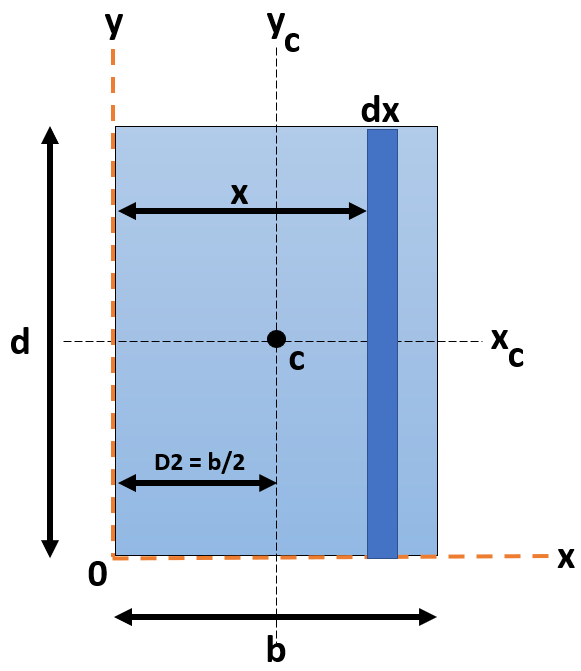
\includegraphics[scale=0.4]{rectangleMOIcorner_Iy.png}
		\end{figure}
		\begin{table}[H]
				\centering
				\begin{tabular}{c|c}
					{$\begin{aligned}
					I_x &= \int_{0}^{d}y^2(bdy) = b\int_0^{d}y^2dy\\
					I_x &= b\left[\dfrac{y^3}{3}\right]_0^{d} = \dfrac{bd^3}{3}
					\end{aligned}$}&
					
					{$\begin{aligned}
					I_y &= \int_{0}^{b}x^2(d(dx)) = d\int_{0}^{b}x^2dx \\
					I_y &= d\left[\dfrac{x^3}{3}\right]_0^{b} = \dfrac{db^3}{3}
					\end{aligned}$}
				\end{tabular}
		\end{table}
		\begin{itemize}
			\item The above can also be solved using Parallel axis theorem, since the axis $I_x$ is parallel to the centroidal axis $I_{x_c}$ and the axis $I_y$ is parallel to the centroidal axis $I_{y_c}$
		\end{itemize}
%-----------------------------------------------------------------------------------------%
	\section{Parallel axis theorem}
		\begin{itemize}
			\item $\boxed{I_x = I_{xc} + Ad_1^2}\;\;\;\boxed{I_y = I_{yc} + Ad_2^2}\;\;\;\boxed{I_{xy} = I_{x_cy_c}+Ad_1d_2}$ 
			\item $d_1$ = Distance of between x-axis and centroidal x-axis
			\item $d_2$ = Distance between y-axis and centroidal y-axis
		\end{itemize}\hrulefill
%-----------------------------------------------------------------------------------------%
	\subsection{Finding Area MOI of rectangle with origin at bottom right corner using Parallel axis theorem}
		\begin{itemize}
			\item We have derived that Area MOI of the rectangle(b*d) about its centroidal axis is:
			\item $\boxed{I_{x_c} = \dfrac{bd^3}{12}}\;\;\;\boxed{I_{y_c} = \dfrac{db^3}{12}}$
			\item Now using the above result, we can find $I_x$ and $I_y$ that is parallel to their respective centroidal axis as follows:
		\end{itemize}
		\begin{table}[H]
			\centering
			\begin{tabular}{c|c}
				${\begin{aligned}
				I_x &= I_{x_c} + Ad_1^2 \impliedby (Here\;d_1=d/2)\\
				I_x &= \dfrac{bd^3}{12} + (b*d)\left(\dfrac{d}{2}\right)^2\\
				I_x &= \dfrac{bd^3}{12} + \dfrac{bd^3}{4}\\
				\implies \Aboxed{I_x &= \dfrac{bd^3}{3}}		
				\end{aligned}}$
				&
				${\begin{aligned}
				I_y &= I_{y_c} + Ad_2^2 \impliedby (Here\;d_2=b/2)\\
				I_y &= \dfrac{db^3}{12} + (b*d)\left(\dfrac{b}{2}\right)^2\\
				I_y &= \dfrac{db^3}{12} + \dfrac{db^3}{4}\\
				\implies \Aboxed{I_y &= \dfrac{db^3}{3}}
				\end{aligned}}$
			\end{tabular}
		\end{table}
		\begin{itemize}
			\item From the above, it is evident how necessary and useful it is to remember the Area MOI of regular shapes about their centroidal axis as it can greatly help in deriving their Area MOI about any axis that is parallel to their centroidal axis. 
		\end{itemize}\hrulefill
%-----------------------------------------------------------------------------------------%	
	\section{Product of Inertia ($I_{xy}$)}
		\begin{itemize}
			\item If $I_{xy} = 0$, then that axis is called \textbf{Principal axis}
			\item Unlike Area MOI, Product of Inertia can be +ve, 0, -ve
			\item Product of Inertia about any symmetrical axis will be zero
			\item $\boxed{I_{xy} = \int xydA}$
		\end{itemize}
		\begin{table}[H]
		\centering
		\begin{tabular}{cc}
			\parbox{5cm}{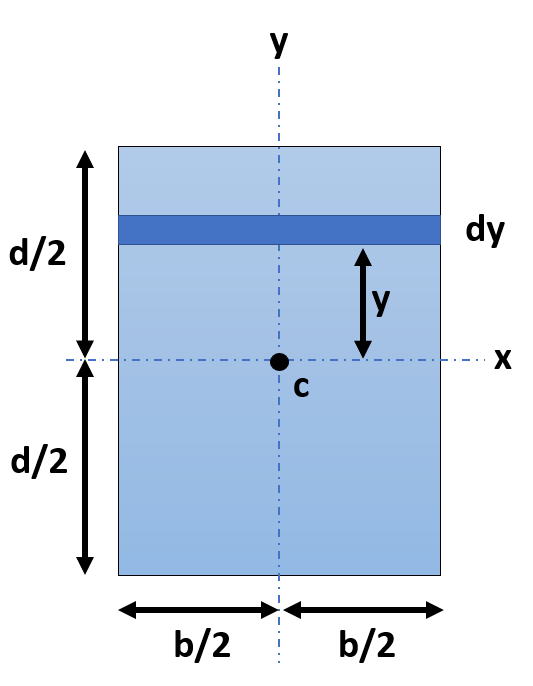
\includegraphics[scale=0.4]{rectangleMOI_Ix.png}} 
			& \parbox{7cm}{
			\begin{align*}
				I_{x_cy_c} &= \int \bar{x}\bar{y}dA = \int_{-d/2}^{d/2} \left(\dfrac{b}{2}\right)y(bdy)\\
				I_{x_cy_c} &= b^2\left[\dfrac{y^2}{2}\right]_{-d/2}^{d/2}\\
				I_{x_cy_c} &= b^2(0) = 0\;\;\;(As\;x_c\;and\;y_c\;are\;Symmetrical\;axis)
			\end{align*}}
		\end{tabular}
	\end{table}\hrulefill
%-----------------------------------------------------------------------------------------%
	\section{Perpendicular axis theorem}
		\begin{itemize}
			\item The Polar moment of Inertia ($I_z$) is based on the perpendicular axis theorem which defines an Area MOI wrt to an axis that is perpendicular to the cross-sectional area
			\item $\boxed{I_z = I_x + I_y}\implies$ $I_z = \int \rho^2dA = \int (x^2+y^2)dA = \int x^2dA + \int y^2dA = I_y + I_x$
			\item It is based on Pythagorean theorem
			\begin{figure}[H]
				\centering
				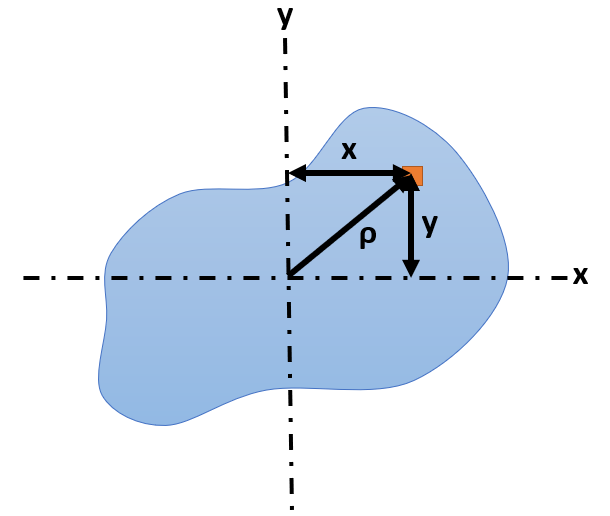
\includegraphics[scale=0.5]{perpendiculartheorem.png}
			\end{figure}
			\item This can be used to calculate indirectly the Area MOI of a circle of radius R about its centroidal axes
		\end{itemize}\hrulefill
%-----------------------------------------------------------------------------------------%
	\subsection{Finding Area MOI of a circle about its centroidal axes using $I_z$}
		\begin{table}[H]
		\centering
		\begin{tabular}{cc}
			\parbox{5cm}{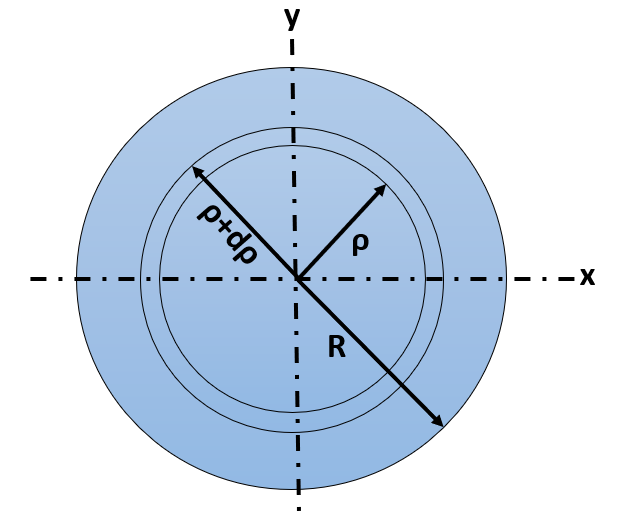
\includegraphics[scale=0.5]{circleMOI.png}} 
			& \parbox{7cm}{
			\begin{align*}
				We\;know,\;I_z&=\int\rho^2dA\\
			Here,\;dA&=\pi(\rho+d\rho)^2-\pi\rho^2 = \pi(\rho^2+(d\rho)^2+2\rho d\rho-\rho^2)\\
			\implies dA &= \pi 2\rho d\rho\\
			I_z &= \int_0^R\rho^2(\pi 2\rho d\rho) = 2\pi\int_0^R\rho^3d\rho\\
			I_z &= 2\pi\left[\dfrac{\rho^4}{4}\right]_0^R = \dfrac{\pi R^4}{2}\\
			I_z &= I_x + I_y \implies  \dfrac{\pi R^4}{2} =  \dfrac{\pi R^4}{4} +  \dfrac{\pi R^4}{4}\\
			So,\;\Aboxed{I_x &= I_y =  \dfrac{\pi R^4}{4} =  \dfrac{\pi D^4}{64}}
			\end{align*}}
		\end{tabular}
	\end{table}\hrulefill
%-----------------------------------------------------------------------------------------%	
	\section{Rotation of Axes}
		\begin{itemize}
			\item $\boxed{I_{x'} = \left(\dfrac{I_x+I_y}{2}\right)+\left(\dfrac{I_x-I_y}{2}\right)cos2\theta-I_{xy}sin2\theta}\;\;\;\boxed{I_{y'} = \left(\dfrac{I_x+I_y}{2}\right)-\left(\dfrac{I_x-I_y}{2}\right)cos2\theta+I_{xy}sin2\theta}$
			\item $\boxed{I_{x'y'} = \left(\dfrac{I_x-I_y}{2}\right)sin2\theta+I_{xy}cos2\theta}$
			\item The above three formulae help us to find the Area MOI of any shape about an axis that is tilted at an anticlockwise angle of $\theta$\textdegree from one of the centroidal axis. 		
		\end{itemize}\hrulefill
%-----------------------------------------------------------------------------------------%
		\subsection{Principal Moment of Inertia($I_1,I_2$)}
			\begin{itemize}
				\item $\boxed{I_1,I_2 = \left(\dfrac{I_x+I_y}{2}\right)\pm\sqrt{\left(\dfrac{I_x-I_y}{2}\right)^2+(I_{xy})^2}}$
				\item Principal MOI denote the maximum($I_1$) and minimum($I_2$) Area MOI of a planar section
				\item The position of these principal Area MOI can be found using:
				\item $\boxed{\theta_{P_1} = \dfrac{tan^{-1}\left(\dfrac{-2I_{xy}}{I_x-I_y}\right)}{2}}\;\;\;\boxed{\theta_{P_2} = \theta_{P_1}+90\deg}$
				\item If an area has axis of symmetry, then product of inertia about those axes will be zero. Hence such axis must be principal axes. \textbf{Symmetrical axis is always principal, but the reverse is not true}
			\end{itemize}\hrulefill
%-----------------------------------------------------------------------------------------%
	\section{Radius of Gyration(k)}
		\begin{itemize}
			\item It is the theoretical distance at which we can condense the entire area of cross section into a narrow strip and have the same Area MOI.
		\item $\boxed{k = \sqrt{\dfrac{I_x}{A}}}$
		\begin{figure}[H]
			\centering
			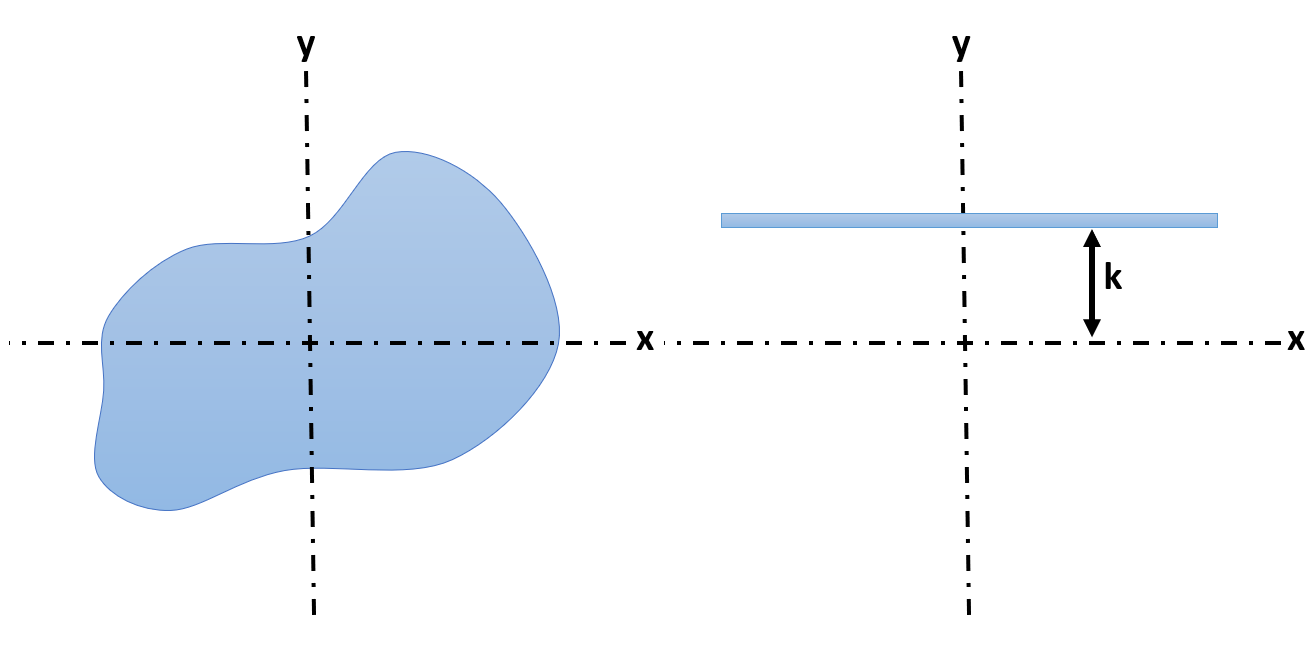
\includegraphics[scale=0.4]{radiusofgyration.png}
		\end{figure}
		\end{itemize}\hrulefill
%-----------------------------------------------------------------------------------------%
\chapter{Bending stresses in Beams}	
	\section{Effect of Bending}
		\begin{itemize}
			\item \textbf{Neutral Axis} : The transverse axis about which the CS area rotates is called Neutral Axis. In pure bending, the NA always passes through the centroid. In plastic bending, NA passes through equal area axis.
			\begin{figure}[H]
				\centering
				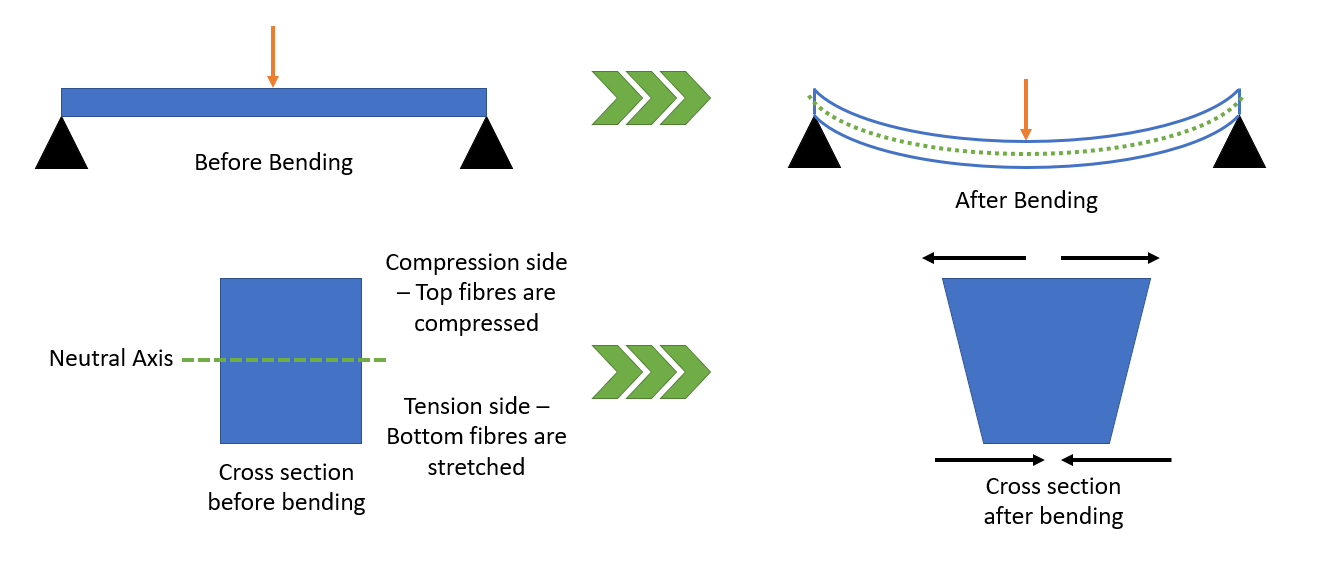
\includegraphics[scale=0.4]{effectofbending.png}
			\end{figure}
			\item Hence, a rectangular section before bending will be trapezoidal section after bending. But such deformations in CS area (called transverse deformations since they are perpendicular to the applied) are very small and so negligible. So for all practical purposes, the CS area can be considered to be rectangular even after bending.
		\end{itemize}\hrulefill
%-----------------------------------------------------------------------------------------%
	\section{Simple bending or Pure bending}
		\begin{itemize}
			\item If the bending moment is constant along a portion of the beam, then that portion is said to be under pure bending. $\implies \dfrac{dM}{dx} = 0 \implies SF = 0$
		\end{itemize}
		\subsection{Assumptions in Theory of pure bending}
			\begin{itemize}
				\item Material is \textbf{Homogeneous, Isotropic and linearly elastic}
				\item The beam is \textbf{Prismatic} and \textbf{straight} before loading
				\item The \textbf{Young's modulus(E) is same for tension and compression}
				\item Plane section before bending remains plane section after bending $\implies$ Longitudinal strain vary linearly from zero at NA to max at the surface. $\boxed{Longitudinal\;strain\propto Distance\;of\;the\;fibre\;from\;NA}$
				\item The section of the beam is symmetrical in the loading plane. If asymmetrical, then twisting and warping may occur along with bending. 
			\end{itemize}\hrulefill
%-----------------------------------------------------------------------------------------%
	\section{Equation of Pure bending}
		\begin{itemize}
			\item[] $$\boxed{\dfrac{M}{I} = \dfrac{\sigma}{y} = \dfrac{E}{R}}$$
			\item R = Radius of curvature
			\item I = Area MOI of CS about NA 
			\item M = Bending Moment
			\item $\sigma$ = Bending stress in a fibre at a distance y from NA
			\item E = Modulus of Elasticity
			\item \textbf{Limitation of Pure bending eqn: }Applicable only in case of pure bending
		\end{itemize}\hrulefill
%-----------------------------------------------------------------------------------------%
	\subsection{Nature of Bending stress}
		\begin{figure}[H]
			\centering
			\includegraphics[scale=0.5]{natureofbending.png}
		\end{figure}
		\begin{itemize}
			\item \fbox{Total compressive force = Average stress * Area under compression}
			\item \fbox{Total Tensile force = Average stress * Area under Tension}
			\item Average stress is nothing but the stress calculated using the pure bending equation. $\boxed{\sigma = \dfrac{M}{I}y}$
		\end{itemize}\hrulefill
%-----------------------------------------------------------------------------------------%
	\section{Section Modulus(Z)}
		\begin{itemize}
			\item Represents the strength of the section
			\item It is the ratio of Area MOI of the beam's Cross section about NA to the distance of the extreme fibre from NA. 
			\item $\implies \boxed{Z = \dfrac{I}{y_{max}}}$ Unit: $mm^3$
			\item If Section modulus is known, then Max Bending stress: $\boxed{\sigma_{max} = \dfrac{M}{Z}}$
		\end{itemize}\hrulefill
%-----------------------------------------------------------------------------------------%
	\section{Moment of Resistance ($M_R$)}
		\begin{itemize}
			\item Represents the Max Bending moment that can be resisted by the section without failure
			\item $\boxed{M_R=\sigma_PZ} \impliedby$ (Valid only for Symmetrical section about NA, $\sigma_P$ = Permissible stres)
			\item If section is asymmetrical (Eg. T section), $\boxed{M_{R_1} = \sigma_cZ_c}$ and $\boxed{M_{R_2} = \sigma_tZ_t}$. The $M_R$ will be the lesser of the two values. 
			\item[$\implies$] $\sigma_c,\sigma_t$ are permissible bending stress in compression and Tension respectively 
		\end{itemize}\hrulefill
%-----------------------------------------------------------------------------------------%
	\section{Bending Stresses in Axially loaded beams}
		\begin{itemize}
			\item Direct Axial Load: $\boxed{\sigma = \pm\dfrac{M}{I}y\pm\dfrac{P}{A}} \impliedby$ (P = Axial load)
			\item Eccentric Axial Load: $\boxed{\sigma = \pm\dfrac{M}{I}y\pm\dfrac{P}{A}\pm\dfrac{Pe}{I}y} \impliedby$ (e = Eccentricity)
		\end{itemize}\hrulefill
%-----------------------------------------------------------------------------------------%	
	\section{Forces on Partial Area of a Section}
		\begin{itemize}
			\item The force on a partial area of a cross section can be found by using similar triangles concept on the stress diagram when Max bending stress($\sigma_{max}$) is known
			\begin{figure}[H]
				\centering
				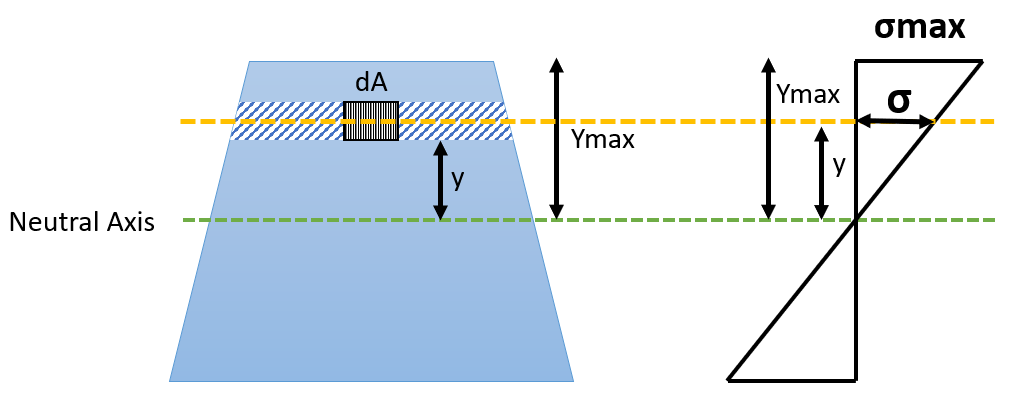
\includegraphics[scale=0.4]{forcepartial.png}
			\end{figure}
			\item From the above diagram, $\boxed{\sigma = \dfrac{\sigma_{max}}{y_{max}}y}$
			\item We know, $Stress=\dfrac{Force}{Area}$. So, Force = Stress * Area
			\item So, $dF = \sigma dA = \dfrac{\sigma_{max}}{y_{max}}ydA \implies$ $F = \dfrac{\sigma_{max}}{y_{max}}\int ydA = \boxed{\dfrac{\sigma_{max}}{y_{max}}A\bar{y}}$
		\end{itemize}\hrulefill
%-----------------------------------------------------------------------------------------%
	\section{Bending stress distribution in Composite Beam}
		\begin{itemize}
			\item If the materials are joined firmly with each other, there will be a common NA
			\item If they are not joined together, then both beam will bend independently about their own NA. Eg. Leaf springs. The Total $M_R$ is this case will be the sum of the two. 
			\item In case of composite beams, the position of NA will not be the centroid of the section as they are made of different materials and hence don't satisfy the condition of pure bending
			\item The composite section can be converted into an equivalent section made of either of the two materials. For that equivalent section, the centroid will coincide with the NA
			\item In composite beams, the bending strain diagram is linear, hence strain in the two materials at a given distance from NA will be the same $\impliedby$ \textbf{Strain compatibility condition}
		\end{itemize}\hrulefill
%-----------------------------------------------------------------------------------------%
	\subsection{Equivalent section}
		\begin{itemize}
			\item \textbf{Modular ratio(m):} = $\dfrac{E_1}{E_2}$
			\begin{figure}[H]
				\centering
				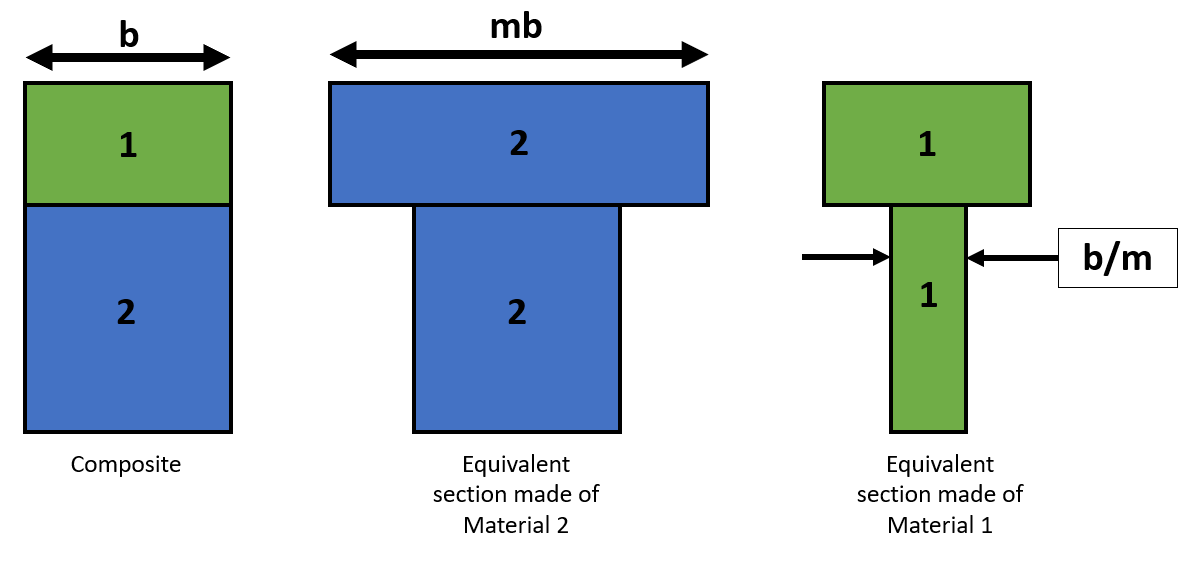
\includegraphics[scale=0.4]{equisection.png}
			\end{figure}
		\end{itemize}\hrulefill
%-----------------------------------------------------------------------------------------%
	\section{Flitched Beam}
		\begin{itemize}
			\item Wooden section strengthened by metal plate either provided at top-and-bottom or at left-and-right symmetrically
			\item Flitched beams are provided when a homogeneous beam of wood will require large cross-sectional area for same moemnt of resistance. 
			\item Generally top-and-bottom flitched beam is 3-5 times stronger than side flitched beam
		\end{itemize}\hrulefill
%-----------------------------------------------------------------------------------------%
	\subsection{Finding $M_R$ of Top and Bottom Flitched beam using Strain compatibility method}
		\begin{figure}[H]
			\centering
			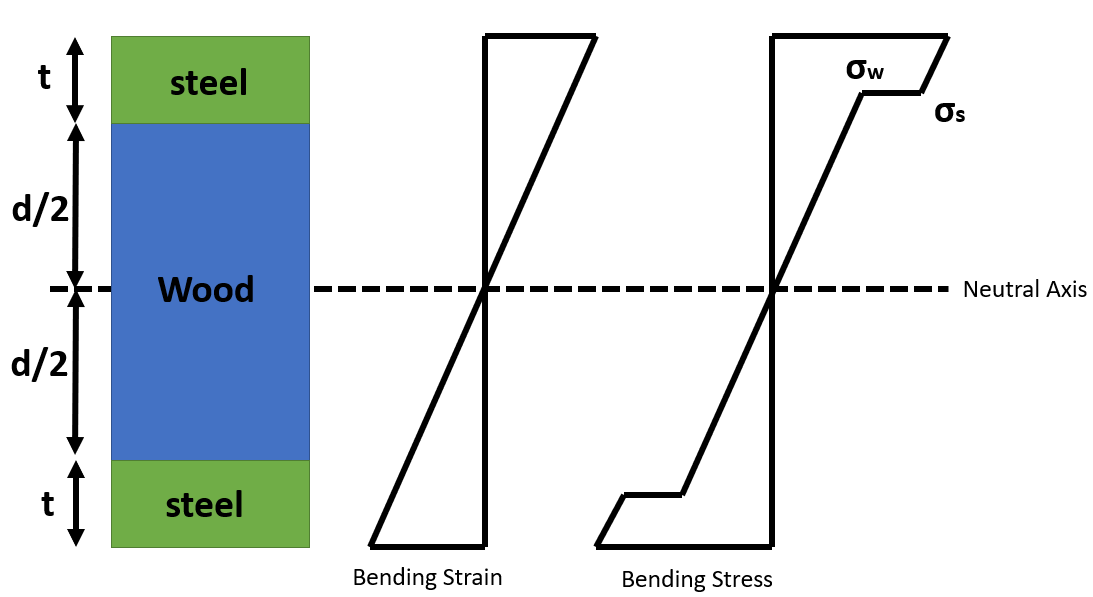
\includegraphics[scale=0.4]{flitchedbeam.png}
		\end{figure}
		\begin{itemize}
			\item For composite beams, by strain compatibility condition: \fbox{Strain in steel = Strain in Wood} $\implies \in_s = \in_w$ 
			\item $\implies \dfrac{\sigma_s}{E_s} = \dfrac{\sigma_w}{E_w} \implies \dfrac{\sigma_s}{\sigma_w} = \dfrac{E_s}{E_w} = m$
			\item[$\implies$] At the same distance from NA, if $\sigma_s$ is the bending stress in steel, then $\sigma_w$ at that level will be $\sigma_s/m$
			\item Let permissible stress in wood be $\sigma_w$. Then Total $M_R = M_{R_W} + M_{R_S}$
			\item $M_{R_W} = \sigma_WZ = \sigma_W\left(\dfrac{I}{y_{max}}\right) \implies \sigma_w\left(\dfrac{bd^3/12}{d/2}\right) =  \sigma_W\dfrac{bd^2}{6}$
			\item $M_{R_S} = M_R$ of Steel of size(b*(d+2t)) - $M_R$ of Steel of size(b*d)
			\item $M_{R_S} = \sigma_{S_{max}}\left(\dfrac{b(d+2t)^3/12}{d/2 + t}\right) - \sigma_S\left(\dfrac{bd^2}{6}\right)$
		\end{itemize}\hrulefill
%-----------------------------------------------------------------------------------------%
	\subsection{Finding $M_R$ of Top and Bottom Flitched beam using Equivalent section method}
		\begin{figure}[H]
			\centering
			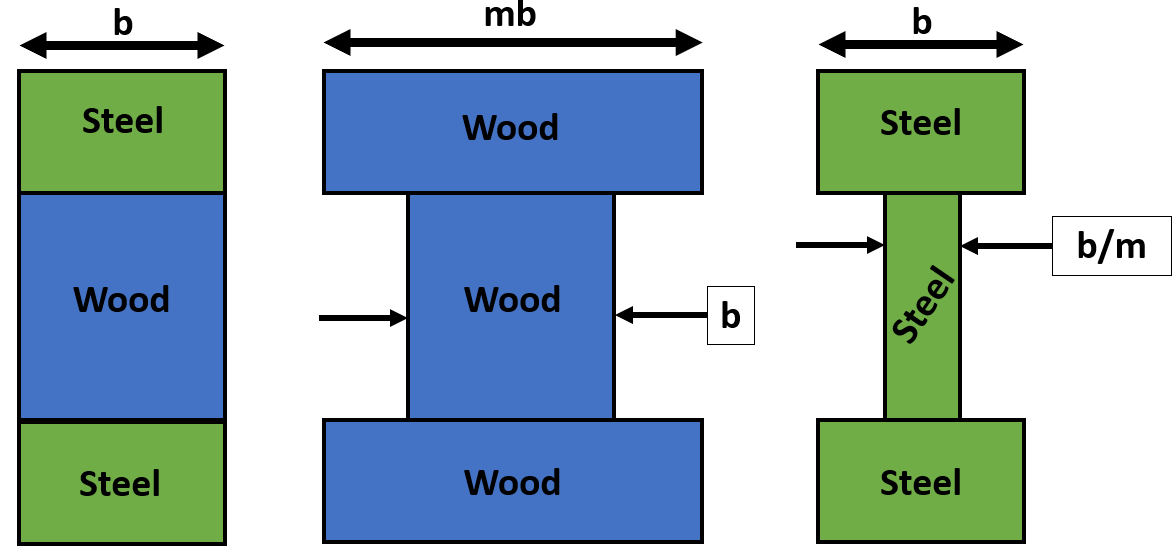
\includegraphics[scale=0.4]{flitchedbeam_MR.png}
		\end{figure}
		\subsubsection{$M_R$ for Equivalent Wood section}
			\begin{align*}
				M_{R} &= \sigma_W\left(\dfrac{I}{y_{max}}\right)\\
				&= \sigma_W.......
			\end{align*}
			\begin{itemize}
				\item $M_R$ (In terms of wood) = $\boxed{\sigma_W\left[\dfrac{mb(d+2t)^2}{6}-\dfrac{(mb-b)d^2}{6}\right]}$
				\item $M_R$ (In terms of steel) = $\boxed{\sigma_s\left[\dfrac{b(d+2t)^2}{6}-\dfrac{b-\dfrac{b}{m}d^2}{6}\right]}$
			\end{itemize}\hrulefill
%-----------------------------------------------------------------------------------------%
	\subsection{Side Flitched Beam}
		\begin{figure}[H]
			\centering
			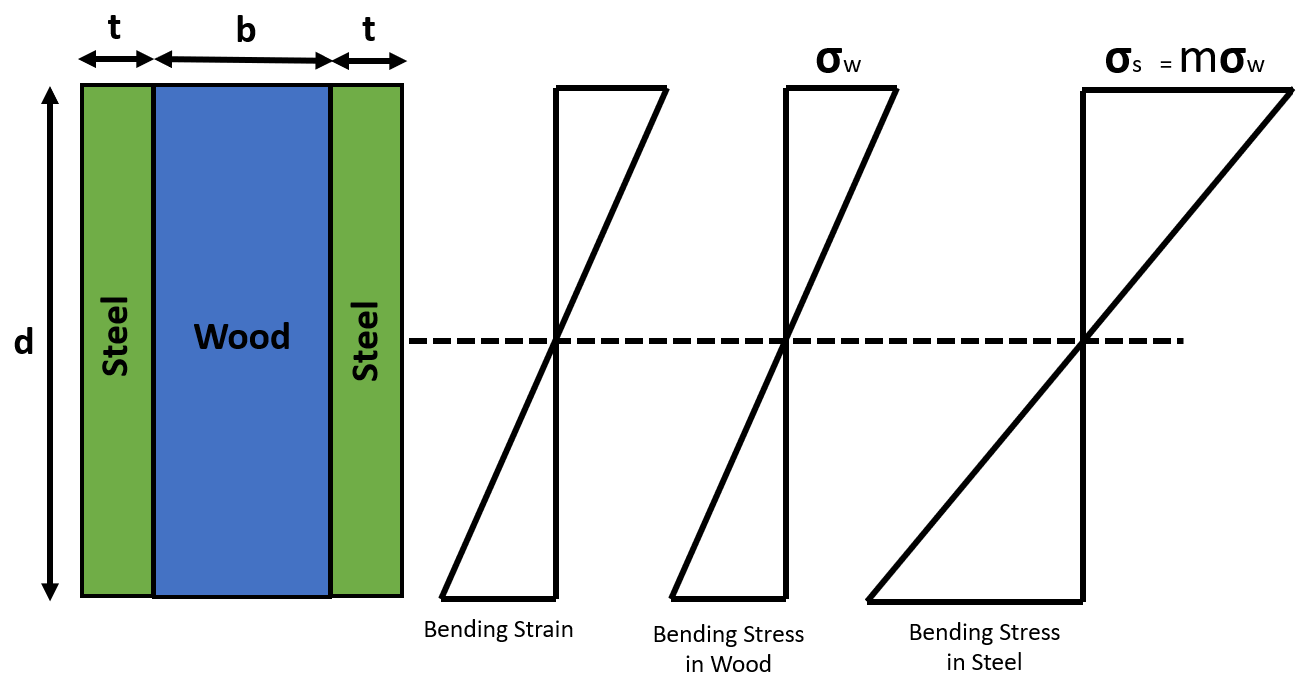
\includegraphics[scale=0.4]{sideflitchedbeam.png}
		\end{figure}
		\begin{itemize}
			\item $\boxed{M_{R_W} = \sigma_W\left(\dfrac{bd^2}{6}\right)}\;\;\;\boxed{M_{R_S} = \sigma_S\left(\dfrac{2td^2}{6}\right)}$
			\item[$\implies$] $\boxed{M_R  = (M_{R_W} + M_{R_S}) = \sigma_W\dfrac{d^2}{6}[b+m2t] = \sigma_S\dfrac{d^2}{6}[\dfrac{b}{m} + 2t]}$			
		\end{itemize}\hrulefill
%-----------------------------------------------------------------------------------------%
	\section{Beam of Uniform Strength}
		\begin{itemize}
			\item For an economical design, the section of the beam may be reduced towards the support, as bending moment decreases towards the support.
		\end{itemize}
	\subsection{Beam of constant width}
		\begin{itemize}
			\item Consider a Simply supported beam AB with cross section (b*d). Section Modulus (Z) of the beam is : $\dfrac{bd^2}{6}$
			\item But for Uniform strength, lets consider that the beam has \textbf{constant width and varying depth} along its length. $\implies Z=\dfrac{bd_x^2}{6} \impliedby (d_x$ = depth of the beam at a distance x from support A). $M_{R_x} = \sigma\dfrac{bd_x^2}{6}$
			\item Just like how we calculate the moment at a distance x ($M_x$) in BMD, $M_x$ will be $\dfrac{Wx}{2}$ for a point load W acting at the center of the beam
			\item $(M_{R_x} = M_x) \implies \sigma\dfrac{bd_x^2}{6} = \dfrac{Wx}{2} \implies \boxed{d_x = \sqrt{\dfrac{3W}{b\sigma}}\sqrt{x}} \impliedby$ (Parabolic)
		\end{itemize}\hrulefill
%-----------------------------------------------------------------------------------------%
	\subsection{Beam of constant depth}
		\begin{itemize}
			\item Similarly let's consider instead of depth, the width is varying. So, $(M_{R_x} = M_x) \implies \sigma\dfrac{b_xd^2}{6} = \dfrac{Wx}{2}$
			\item[$\implies$] $\boxed{b_x = \dfrac{3Wx}{\sigma d^2}}\impliedby$ (Linear)
		\end{itemize}\hrulefill
%-----------------------------------------------------------------------------------------%
	\section{Biaxial Bending}
		\begin{itemize}
			\item 
		\end{itemize}\hrulefill
%-----------------------------------------------------------------------------------------%
\chapter{Shear stresses in Beams}
	\section{Shear stress distribution in Beams}
		\begin{itemize}
			\item \textbf{Assumptions:}
				\begin{itemize}
					\item Material is Homogeneous, elastic
					\item Obeys Hooke's Law
					\item Shear stress($\tau$) is assumed constant along width and variation along depth
				\end{itemize}
			\item $\boxed{\tau = \dfrac{SA\bar{y}}{Ib}}$
			\item S = Shear force at any section
			\item A$\bar{y}$ = Area MOI of section above y about NA
			\item $\bar{y}$ = Distance from centroid of area above y to NA
			\item I = Area MOI of the whole section about NA
			\item b = Width of the section at a distance y from NA
		\end{itemize}\hrulefill
%-----------------------------------------------------------------------------------------%
	\section{Shear Stress distribution}
	\textsc{Steps to find the Shear stress distribution for any cross section}
		\begin{itemize}
			\item Find the terms in the formula $\boxed{\dfrac{SA\bar{y}}{Ib}}$ for the given cross sectionf
			\item Equate $\dfrac{d\tau}{dy}=0$ to find the value of y for which $\tau$ is max.
			\item Then see if $\tau_{max}$ can be equated to $\tau_{avg}$ which is $\dfrac{S}{Area\;of\;whole\;section}$
			\item Equate $\tau$ with $\tau_{avg}$ to find the value of y where $\tau_{avg}$ occurs				
		\end{itemize}\hrulefill
%-----------------------------------------------------------------------------------------%
	\subsection{Shear stress distribution in Rectangular section}
		\begin{figure}[H]
			\centering
			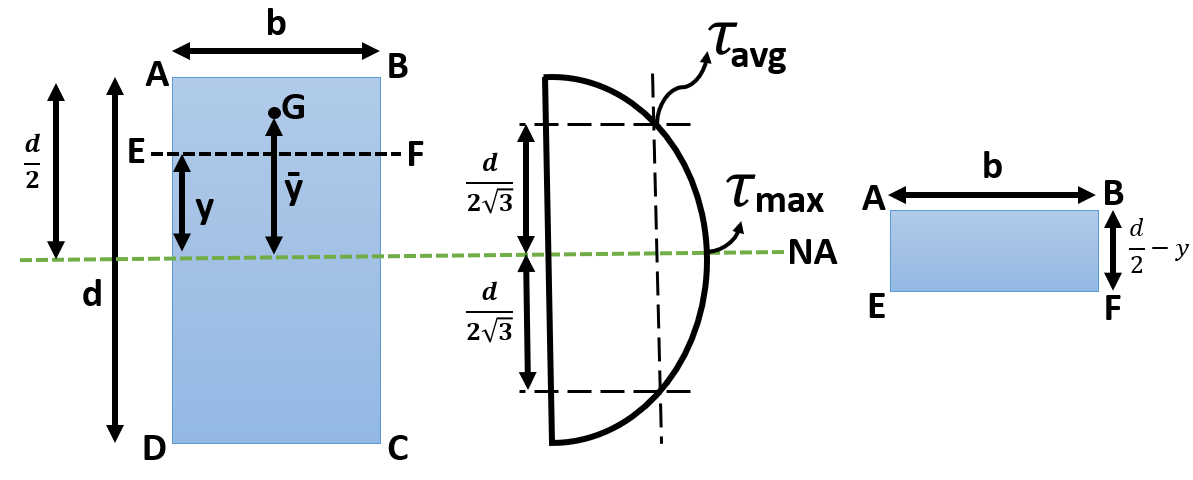
\includegraphics[scale=0.4]{shearstressdistribution_rectangle.png}
		\end{figure}
		\begin{itemize}
			\item We know, $\boxed{\tau = \dfrac{SA\bar{y}}{Ib}}$
			\item Here, Area of ABEF (A) = $b\left(\dfrac{d}{2}-y\right)$
			\item $\bar{y} = y + \dfrac{(\dfrac{d}{2}-y)}{2} = \dfrac{2y + \dfrac{d}{2} -y}{2} = \dfrac{4y+2-2y}{4} = \dfrac{2y+d}{4} = \dfrac{2(y+\dfrac{d}{2})}{2*2} \implies \boxed{\bar{y}=\dfrac{\left(y+\dfrac{d}{2}\right)}{2}}$
			\item Area MOI of whole section about NA (I) = $\dfrac{bd^3}{12}$
			\item[$\implies$] $\tau = \dfrac{S*\left(b\left(\dfrac{d}{2}-y\right)\right)\left(\dfrac{d}{2}+y\right)}{2\left(\dfrac{bd^3}{12}\right)b} \implies \boxed{\tau = \dfrac{6S}{bd^3}\left(\dfrac{d^2}{4}-y^2\right)} \impliedby$ (Parabolic variation)
			\item From the above result, we can infer that $\tau = 0$ when y = $\pm\dfrac{d}{2}$ and for $\tau_{max},\;\;\dfrac{d\tau}{dy} = 0$
			\item $\dfrac{d\tau}{dy} = 0 \implies \dfrac{d}{dy}\left[\dfrac{6S}{bd^3}\left(\dfrac{d^2}{4}-y^2\right)\right] = 0 \implies \dfrac{-12Sy}{bd^3} = 0 \implies \boxed{\tau_{max}\;at\;(y=0)}$
			\item $\implies \boxed{\tau_{max} = \dfrac{3S}{2bd}} \impliedby$ (Here, $\dfrac{S}{bd} = \dfrac{S}{A} = \tau_{avg}) \implies \boxed{\tau_{max} = \dfrac{3}{2}\tau_{avg}}$
			\item Now, to find the distance at which $\tau_{avg}$ occurs, let $\tau = \tau_{avg}$
			\item[$\implies$] $\dfrac{6S}{bd^3}\left(\dfrac{d^2}{4}-y^2\right) = \dfrac{S}{bd}\;\;\;$ Solving this, will give $\boxed{y = \pm\dfrac{d}{2\sqrt{3}}}$
		\end{itemize}\hrulefill
%-----------------------------------------------------------------------------------------%
	\subsection{Shear Stress distribution in Triangular section}
		\begin{itemize}
			\item $\boxed{\tau_{max} = \dfrac{3S}{bh}}\;\;\;\boxed{\tau_{max} = \dfrac{3}{2}\tau_{avg}}$
			\item Shear stress at centroid is $\dfrac{4}{3}$ times the Avg Shear stress
			\item $\tau_{max}$ occurs at h/2. but NA is at h/3. So unlike the rectangular section for which the max shear occurs at NA, triangular section is different. 
			\item $\tau_{avg}$ occurs at ???
		\end{itemize}\hrulefill
%-----------------------------------------------------------------------------------------%
	\subsection{Shear Stress distribution in Circular section}
		\begin{itemize}
			\item $\boxed{\tau_{max} = \dfrac{4S}{3\pi R^2}}\;\;\;\boxed{\tau_{max} = \dfrac{4}{3}\tau_{avg}}$
			\item Shear stress at centroid is $\dfrac{4}{3}$ times the Avg Shear stress
			\item $\tau_{max}$ occurs at NA
			\item $\tau_{avg}$ occurs at $\pm\dfrac{R}{2}$
		\end{itemize}\hrulefill
%-----------------------------------------------------------------------------------------%
	\subsection{Shear Stress distribution in I-section}
		\subsubsection{Shear stress distribution in Flange}
			\begin{itemize}
				\item
			\end{itemize}
		\subsubsection{Shear stress distribution in Web}
			\begin{itemize}
				\item
			\end{itemize}\hrulefill
%-----------------------------------------------------------------------------------------%
	\section{Shear stresses in composite sections}
		\begin{itemize}
			\item Convert the given section into its equivalent section of any one material using the \textbf{modular ratio (m)} and then apply the formula $\dfrac{SA\bar{y}}{Ib}$
		\end{itemize}\hrulefill
%-----------------------------------------------------------------------------------------%
	\section{Shear Center}
		\begin{itemize}
			\item For transverse load acting on the plane of symmetry of a a symmetrical cross section beam, the beam will bend without twisting. 
			\item But that's not the case with asymmetrical beam. For symmetrical beam to bend without twisting, the load must act at a point called \textbf{Shear center}
		\end{itemize}\hrulefill
%-----------------------------------------------------------------------------------------%
	\section{Shear stress distribution in Thin walled open cross sections}
		\begin{itemize}
			\item
		\end{itemize}\hrulefill
%-----------------------------------------------------------------------------------------%
	\subsection{Shear stresses in wide flange beams}
		\begin{itemize}
			\item
		\end{itemize}\hrulefill
%-----------------------------------------------------------------------------------------%
	\subsection{Shear stresses in Channel section}
		\begin{itemize}
			\item
		\end{itemize}\hrulefill
%-----------------------------------------------------------------------------------------%
	\subsection{Shear stresses in Angle section}
		\begin{itemize}
			\item
		\end{itemize}\hrulefill
%-----------------------------------------------------------------------------------------%
	\subsection{Shear stresses in Z-Section}
		\begin{itemize}
			\item
		\end{itemize}\hrulefill
%-----------------------------------------------------------------------------------------%
\chapter{Principal Stress-Strain \& Failure Theories}
	\section{Principal stress and Principal planes}
		\begin{itemize}
			\item \textbf{Principal Plane: }A plane in which only Normal stresses are acting and Shear stresses are zero
			\item \textbf{Principal stress: }Normal stresses acting on mutually perpendicular planes on which shear stresses are zero
			\begin{itemize}
				\item \textbf{Major Principal stress($\sigma_1$): }Max value of such normal stress
				\item \textbf{Major Principal stress($\sigma_2$): }Min value of such normal stress
			\end{itemize}\hrulefill
		\end{itemize}
%-----------------------------------------------------------------------------------------%
	\section{Methods to find Principal planes and Principal stresses}
		\begin{enumerate}
			\item Analytical method
			\item Graphical method (Mohr's circle)
		\end{enumerate}\hrulefill			
%-----------------------------------------------------------------------------------------%
	\section{Four cases of Stress combinations}
		\begin{enumerate}
			\item Member subjected to Uni-axial stress
			\item Member subjected to Bi-axial stress in mutually perpendicular directions
			\item Member subjected to pure shear stresses
			\item Member subjected to Bi-axial stresses in mutually perpendicular directions as well as shear stresses
		\end{enumerate}\hrulefill
%-----------------------------------------------------------------------------------------%
	\section{Analytical method to solve for Principal stresses \& Principal planes}
	\subsection{Stress analysis in Member subjected to Uni-axial stress}
		\begin{itemize}
			\begin{figure}[H]
				\centering
				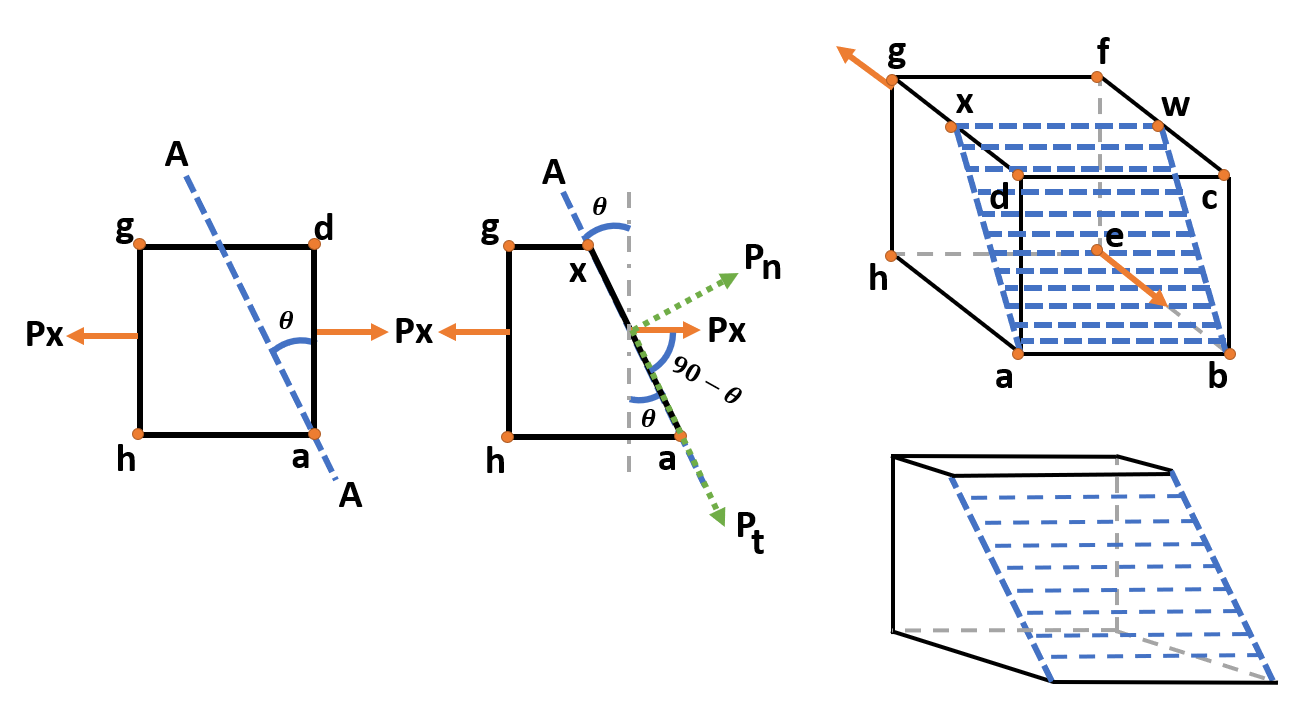
\includegraphics[scale=0.5]{case1.png}
			\end{figure}						
			\item Normal stress due to the force $P_x$ acting on $A_{abcd} = \sigma_x = \dfrac{Px}{A_{abcd}}$
			\item But what is the normal stress acting on an oblique plane like (abwx) ?
			\item Let the normal stress acting on the oblique plane (abwx) be $\sigma_{ob} \implies \sigma_{ob} = \dfrac{P_n}{A_{abwx}}$ 
			\item The force $P_x$ is resolved into two components. $P_n$ is the normal force acting on the oblique plane (abwx) and $P_t$ is the tangential force acting along the oblique plane (abwx)
			\item By resolution of $P_x$, $\boxed{P_n = P_x\sin(90-\theta) = P_x\cos\theta}\;\;\;\boxed{P_t = P_x\cos(90-\theta) = P_x\sin\theta}$
			\item $\cos\theta = \dfrac{A_{abcd}}{A_{abwx}} \implies \boxed{A_{abwx} = \dfrac{A_{abcd}}{Cos\theta}}$
		  \item So, The normal stress ($\sigma_{ob}$) acting on the plane (abwx) is given by: $$\boxed{\sigma_{ob} = \dfrac{P_n}{A_{abwx}} = \dfrac{P_x\cos\theta}{\sfrac{A_{abcd}}{\cos\theta}} = \dfrac{P_x\cos^2\theta}{A_{abcd}} \implies \boxed{\sigma_{ob} = \sigma_{x}\cos^2\theta}}$$
		  \item $\sigma_{ob}$ is max when $\theta$ is 0\textdegree , 180\textdegree ... $\impliedby$ (Because at these angles Cos is max)
		  \item[$\implies$] \fbox{\textbf{Principal stresses:} $\pm\sigma_x \implies \boxed{+\sigma_x=\sigma_1}\;\;\&\;\;\boxed{-\sigma_x=\sigma_2}$}
		  \item Similarly, Tangential stress ($\tau_{ob}$) acting along the plane (abwx) is given by: $$\boxed{\tau_{ob} = \dfrac{P_t}{A_{abwx}} = \dfrac{P_x\sin\theta}{\sfrac{A_{abcd}}{\cos\theta}} = \dfrac{P_x\sin\theta \cos\theta}{A_{abcd}} \implies \boxed{\tau_{ob} = \dfrac{\sigma_x}{2}\sin 2\theta}}$$
		  \item $\tau_{ob}$ is max when $\theta$ is 45\textdegree , 135\textdegree ... $\impliedby$ (Because at these angles $\sin 2\theta$ is max) $\implies\boxed{\tau_{max} = \pm\dfrac{\sigma_x}{2}}$
		  \item Value of Normal stresses in the plane of Maximum shear stress: 
		  \item[]  $\sigma_{ob} = \sigma_x\cos^2$(45\textdegree or 135\textdegree)$\implies \sigma_x\left(\dfrac{1}{\sqrt{2}}\right)^2$ or $\sigma_x\left(\dfrac{-1}{\sqrt{2}}\right)^2\implies \boxed{\sigma_{ob}=\dfrac{\sigma_x}{2}}$
		  \item[$\implies$] \textbf{Magnitude of normal and shear stress is same in the plane of Max shear stress under Uni-axial loading}
		\end{itemize}\hrulefill
%-----------------------------------------------------------------------------------------%
	\subsection{Strain analysis of element subjected to Uni-axial stress}
		\begin{itemize}
			\begin{figure}[H]
				\centering
				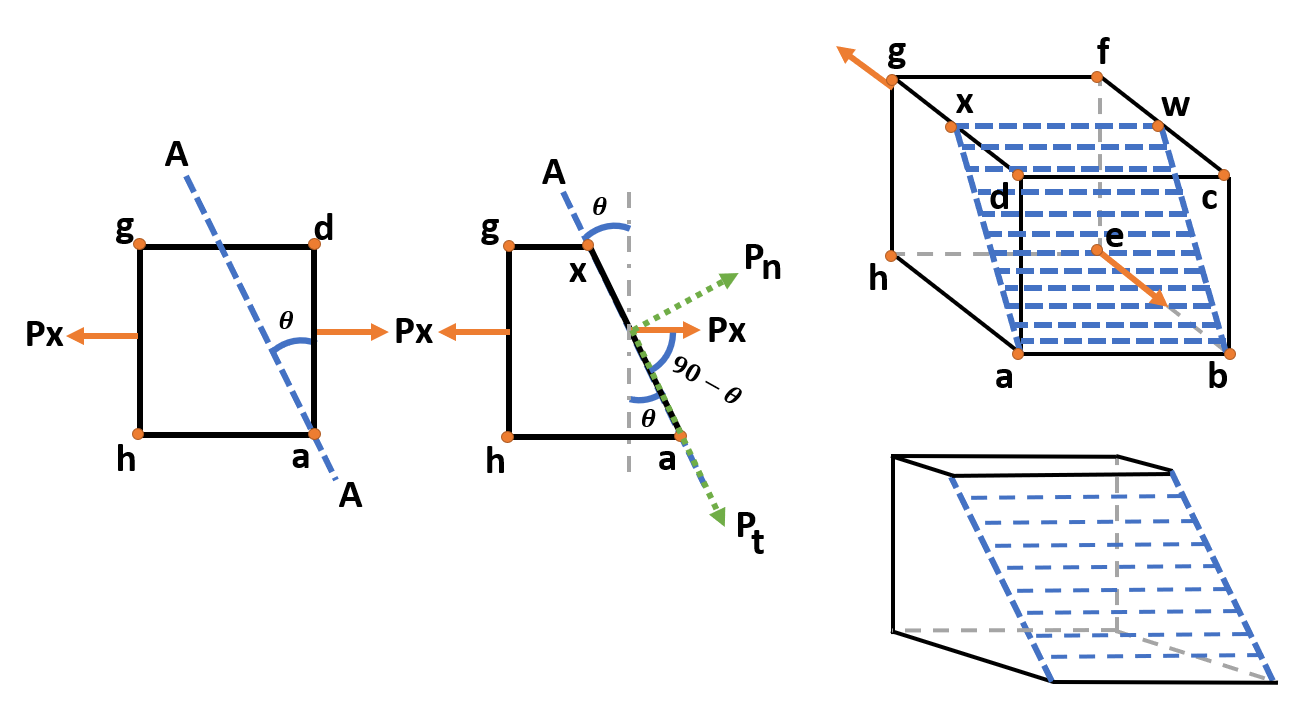
\includegraphics[scale=0.4]{case1.png}
			\end{figure}
			\item We know $\boxed{\sigma_{ob} = \sigma_{x}\cos^2\theta}$ and $\boxed{\tau_{ob} = \dfrac{\sigma_x}{2}\sin 2\theta}$
			\item For principal stress: $\cos^2\theta$ should be max. So $\theta$ will can 0\textdegree , 180\textdegree . If $\theta$ is either of these two values, then $\tau_{ob}$ will be zero. $\implies$ \textbf{Shear stresses will be zero in principal planes for Uni-axial loading}
			\item[$\implies$] \fbox{Principal stresses: $\pm\sigma_x \implies \boxed{+\sigma_x=\sigma_1}\;\;\&\;\;\boxed{-\sigma_x=\sigma_2}$}
			\item \textbf{strain due to to the principal stress($\sigma_x,-\sigma_x$) will be the Principal strain($\in_1,\in_2$)}
			\item \fbox{\textbf{Principal strains} $\implies \boxed{\in_1 = \dfrac{\sigma_1}{E}}$ and $\boxed{\in_2 = \dfrac{-\mu\sigma_1}{E}}$} $\impliedby$ (where $\mu$ is Poisson's ratio of the material)
			\item Let $\in_{ob}$ be the normal strain for any plane and $\phi_{ob}$ be the shear strain for any plane. 
			\item $\boxed{\pmb{\in_{ob}\;=\;\dfrac{\sigma_{ob}}{E}\;=\;\dfrac{\sigma_x\cos^2\theta}{E}\;=\;\in_x\cos^2\theta}}$ and $\boxed{\pmb{\dfrac{\phi_{ob}}{2} = \dfrac{\in_x}{2}\sin 2\theta}}$
			\item The strain formulae can be easily recovered from stress formulae. Just change, $\sigma\rightarrow\in$ and $\tau\rightarrow\dfrac{\phi}{2}$ 
		\end{itemize}\hrulefill
%-----------------------------------------------------------------------------------------%
	\subsection{Stress analysis of member subjected to Bi-axial stress in mutually perpendicular direction}
		\begin{figure}[H]
				\hspace{-0.7cm}
				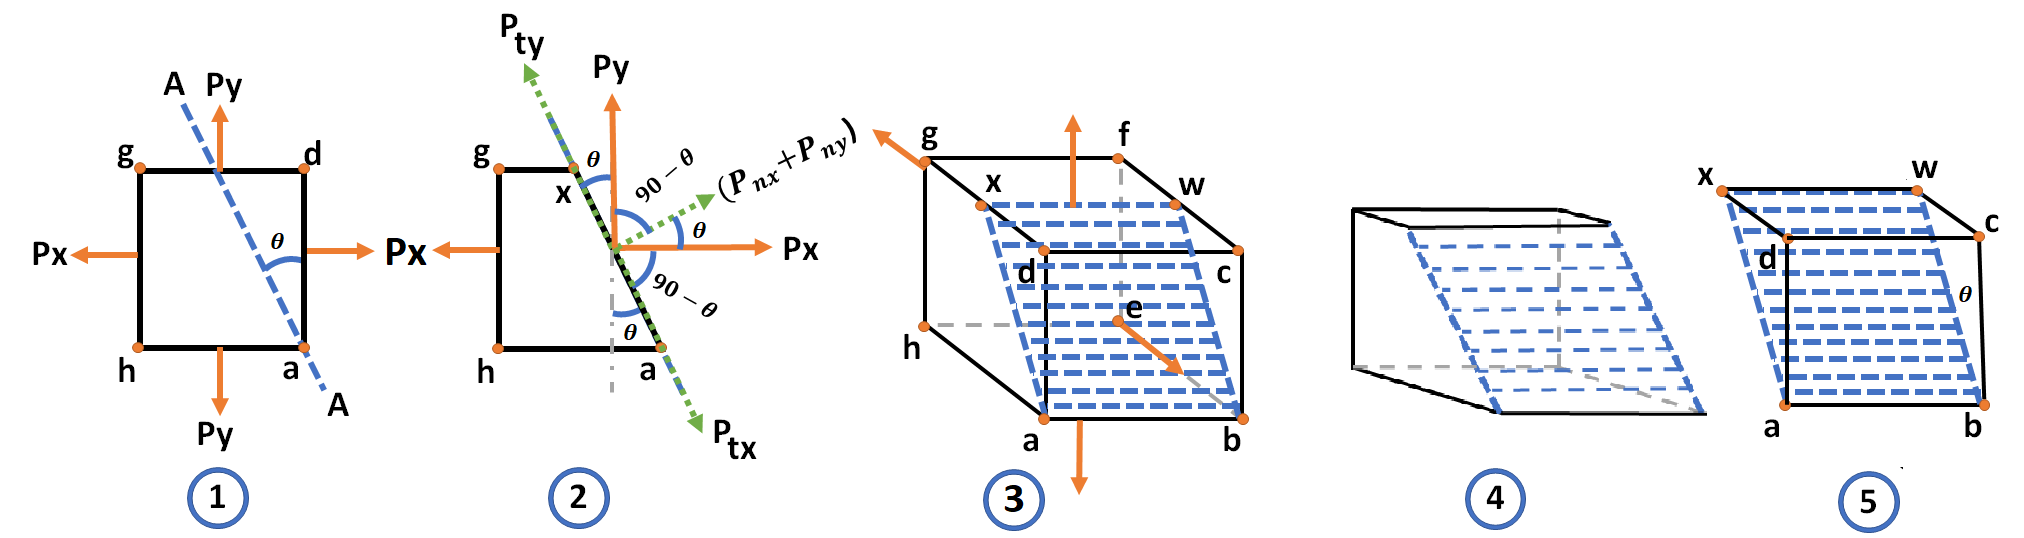
\includegraphics[scale=0.45]{case2a.png}
		\end{figure}
		\begin{itemize}
			\item From Diagram(5) above, $\boxed{\sin\theta = \dfrac{A_{dcwx}}{A_{abwx}}}_{(1)}\;\;\;\boxed{\cos\theta = \dfrac{A_{abcd}}{A_{abwx}}}_{(2)}$	
			\item $\boxed{\sigma_x=\dfrac{P_x}{A_{abcd}}}_{(3)}\;\;\;\boxed{\sigma_y = \dfrac{P_y}{A_{cdwx}}}_{(4)}\;\;\;\boxed{\tau=\dfrac{P_y}{A_{abcd}}}_{(5)}\implies\boxed{P_x=\sigma_x A_{abcd}}_{(6)}\;\;\;\boxed{P_y=\sigma_y A_{dcwx}}_{(7)}$
			\item From Diagram(2):
			\begin{itemize}
				\item Resolving $P_x$ into $P_{nx}$ and $P_{tx} \implies \boxed{P_{nx} = P_x\sin(90-\theta) = P_x\cos\theta}\;\;\;\boxed{P_{tx} = P_x\cos(90-\theta) = P_x\sin\theta}$
				\item Resolving $P_y$ into $P_{ny}$ and $P_{ty} \implies \boxed{P_{ny} = P_y\cos(90-\theta) = P_y\sin\theta}\;\;\;\boxed{P_{ty} = P_y\sin(90-\theta) = P_y\cos\theta}$
			\end{itemize}								
			\item $\sigma_{ob} = \dfrac{P_x\cos\theta + P_y\sin\theta}{A_{abwx}} = \dfrac{\sigma_xA_{abcd}\cos\theta + \sigma_yA_{dcwx}\sin\theta}{A_{abwx}} = \dfrac{\sigma_xA_{abcd}\cos\theta}{A_{abwx}}+\dfrac{\sigma_yA_{dcwx}\sin\theta}{A_{abwx}}$ (Using (6) \& (7))
			\item[$\implies$] (Using (1) \& (2)) $\sigma_x\cos^2\theta + \sigma_y\sin^2\theta = \sigma_x\left[\dfrac{1+\cos 2\theta}{2}\right] + \sigma_y\left[\dfrac{1-\cos 2\theta}{2}\right] = \dfrac{\sigma_x}{2}+\dfrac{\sigma_x\cos 2\theta}{2}+\dfrac{\sigma_y}{2}-\dfrac{\sigma_y\cos 2\theta}{2}$ 
			\item[] $$\implies \boxed{\pmb{\sigma_{ob} = \left(\dfrac{\sigma_x+\sigma_y}{2}\right)+\left(\dfrac{\sigma_x-\sigma_y}{2}\right)\cos 2\theta}}\;...\;Eqn(1)$$
			\item Eqn(1) above is maximum for when $\theta$ = 0\textdegree ,90\textdegree . So, \fbox{\textbf{Principal stress:} $\pmb{\sigma_{1,2} = \left(\dfrac{\sigma_x+\sigma_y}{2}\right)\pm\left(\dfrac{\sigma_x-\sigma_y}{2}\right)}$}
			\item $\tau_{ob} = \dfrac{P_y\cos\theta-P_x\sin\theta}{A_{abwx}} = \dfrac{\sigma_yA_{dcwx}\cos\theta}{A_{abwx}}-\dfrac{\sigma_xA_{abcd}\sin\theta}{A_{abwx}} = \sigma_y\sin\theta\cos\theta - \sigma_x\sin\theta\cos\theta$ (Using (1) \& (2))
			\item[] $$\implies \boxed{\tau_{ob} = (\sigma_x-\sigma_y)\sin\theta\cos\theta = \pmb{\left(\dfrac{\sigma_x-\sigma_y}{2}\right)\sin 2\theta}}\;...\;Eqn(2)$$
			\item Eqn(2) above is maximum for when $\theta$=45\textdegree or 135\textdegree So, Maximum shear stress: $\boxed{\pmb{\tau_{max} = \left(\dfrac{\sigma_x-\sigma_y}{2}\right)}}$
			\item Value of normal stress in the plane of $\tau_{max}$ is $\boxed{\sigma_{ob}=\left(\dfrac{\sigma_x+\sigma_y}{2}\right)} \implies$ \textbf{Normal stresses on the plane of} $\pmb{\tau_{max}}$ \textbf{are equal and alike}. Meaning they are the same for both $\theta$=45\textdegree ,135\textdegree. As $\cos 2\theta$ is zero for both these angles.
			\item Resultant stress on the plane of $\tau_{max}$ is $\sigma_r = \sqrt{\sigma_{ob}^2+\tau_{max}^2} = \sqrt{\left(\dfrac{\sigma_x+\sigma_y}{2}\right)^2+\left(\dfrac{\sigma_x-\sigma_y}{2}\right)^2} = \sqrt{\dfrac{\sigma_x^2+\sigma_y^2}{2}}$
			\item \textbf{Angle of obliquity($\beta$)} : The angle between $\sigma_{ob}$ and $\sigma_r \implies \boxed{\tan\beta=\dfrac{\tau_{max}}{\sigma_{ob}} = \dfrac{\sigma_x-\sigma_y}{\sigma_x+\sigma_y}}$
		\end{itemize}\hrulefill
%-----------------------------------------------------------------------------------------%
	\subsection{Strain analysis of member subjected to Bi-axial stress in mutually perpendicular direction}
		\begin{itemize}
			\begin{figure}[H]
				\hspace{-0.7cm}
				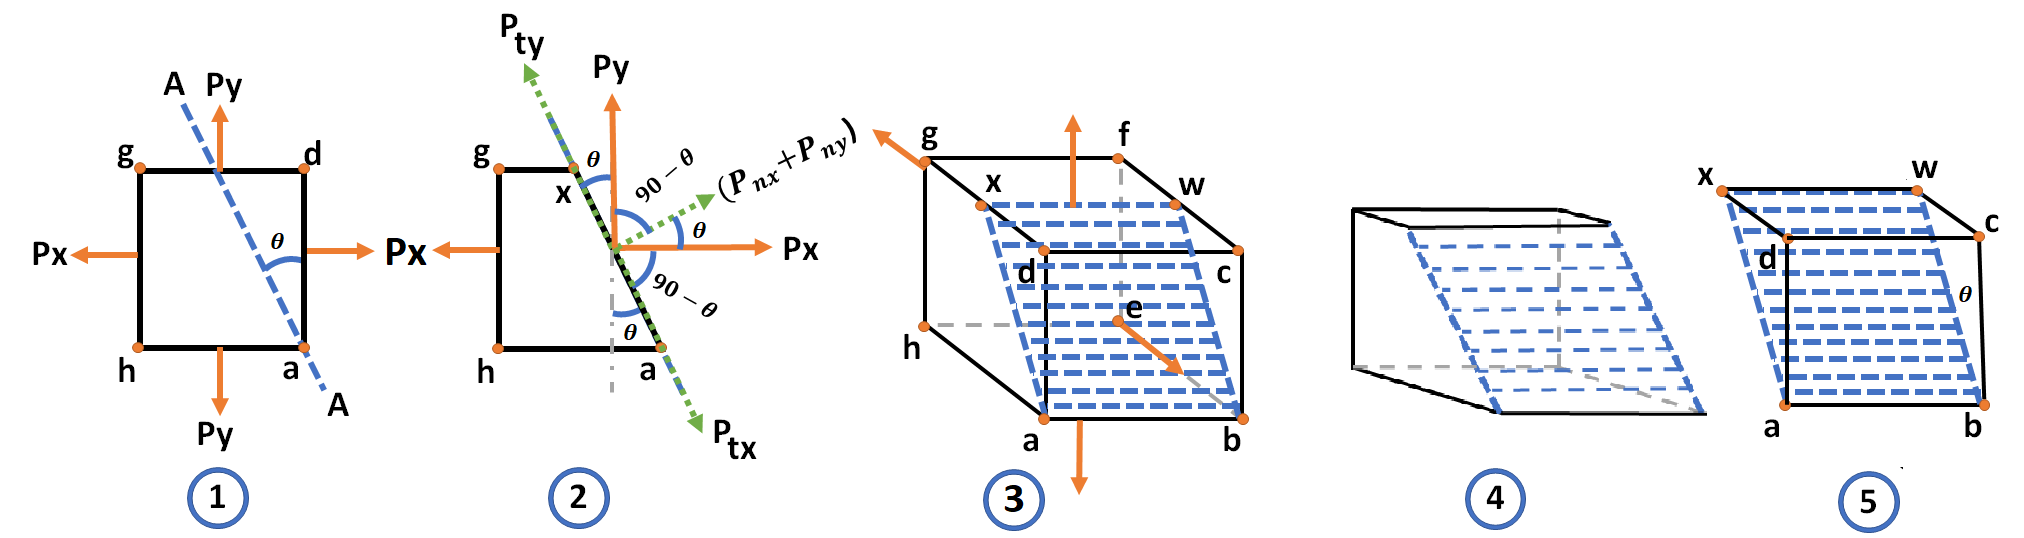
\includegraphics[scale=0.45]{case2a.png}
				\end{figure}						
			\item We know Principal Stress: $\sigma_{1,2} = \left(\dfrac{\sigma_x+\sigma_y}{2}\right)\pm\left(\dfrac{\sigma_x-\sigma_y}{2}\right)$. 
			\item So, \fbox{\textbf{Principal Strain} ($\in_{1,2})= \left(\dfrac{\in_x+\in_y}{2}\right)\pm\left(\dfrac{\in_x-\in_y}{2}\right)$}
			\item Similarly, Maximum Shear stress: $\tau_{max} = \left(\dfrac{\sigma_x-\sigma_y}{2}\right)$ So, \fbox{Maximum Shear strain: $\phi_{ob} = (\in_x-\in_y)$} ($\tau = \phi /2$) 
		\end{itemize}\hrulefill
%-----------------------------------------------------------------------------------------%
	\subsection{Stress analysis of member subjected to Pure shear stresses}
		\begin{figure}[H]
			\centering
			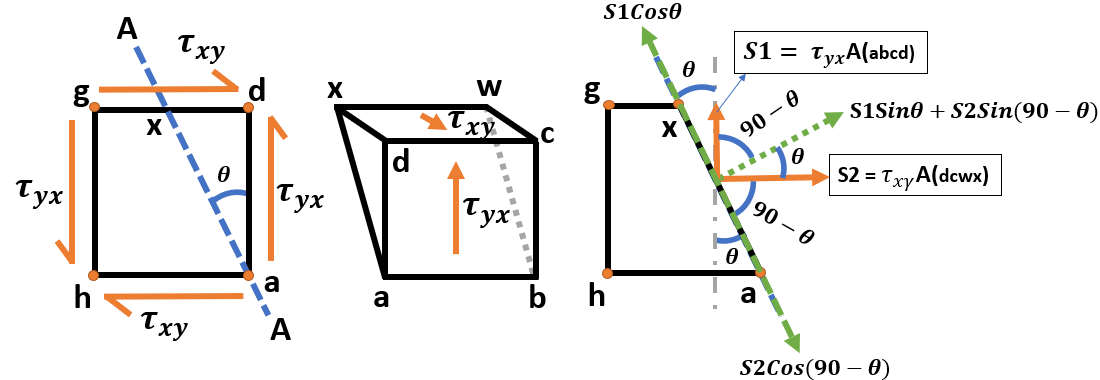
\includegraphics[scale=0.55]{case_pureshear.png}
		\end{figure}
		\begin{itemize}
			\item $\boxed{\sigma_{ob} = \tau_{xy}\sin 2\theta} \impliedby$ Maximum for when $\theta$=45\textdegree , 135\textdegree $\implies$ \fbox{\textbf{Principal Stress:} $\sigma_{1,2} = \pm\tau_{xy}$}
			\item $\boxed{\tau_{ob} = \tau_{xy}\cos 2\theta}\impliedby$ Maximum for when $\theta$=0\textdegree , 90\textdegree $\implies \boxed{\tau_{max} = \pm\tau_{xy}}$ 
			\item Normal stress in the plane of Max shear stress will be Equal and Unlike ${\sigma_{ob} = \pm\tau_{xy}}$ 
		\end{itemize}\hrulefill
%-----------------------------------------------------------------------------------------%
	\subsection{Strain analysis of member subjected to pure shear}
		\begin{itemize}
			\item $\boxed{\in_{ob} = \dfrac{\tau_{xy}\sin 2\theta}{E}}\;\;\;$\fbox{Principal strain: $\in_{1,2} = \dfrac{\pm\tau_{xy}}{E}$}
			\item $\boxed{\dfrac{\phi_{ob}}{2} = \dfrac{\tau_{xy}\cos 2\theta}{G}}\;\;\;$\fbox{Maximum Shear strain: $\dfrac{\phi_{max}}{2} = \dfrac{\pm\tau_{xy}}{G}$} Where G = Shear modulus
		\end{itemize}\hrulefill
%-----------------------------------------------------------------------------------------%
	\subsection{Stress analysis of member subjected to Bi-axial stress in mutually perpendicular direction as well as shear stresses}
		\begin{itemize}
			\item $\boxed{\sigma_{ob} = \left(\dfrac{\sigma_x+\sigma_y}{2}\right)\pm \left(\dfrac{\sigma_x-\sigma_y}{2}\right)\cos 2\theta+\tau_{xy}\sin 2\theta}\;\;\;\boxed{\tau_{ob} = -\left(\dfrac{\sigma_x-\sigma_y}{2}\right)\sin 2\theta+\tau_{xy}\cos 2\theta}$
			\item To find principal plane, Equate $\tau_{ob} = 0 \implies \boxed{\tan 2\theta_p = \dfrac{2\tau_{xy}}{\sigma_x-\sigma_y}}$
			\item \fbox{\textbf{Principal stresses:} $\pmb{\sigma_1,\sigma_2 = \left(\dfrac{\sigma_x+\sigma_y}{2}\right)\pm\sqrt{\left(\dfrac{\sigma_x-\sigma_y}{2}\right)^2+\tau_{xy}^2}}$}
		\end{itemize}\hrulefill
%-----------------------------------------------------------------------------------------%
	\subsection{Strain analysis of member subjected to Bi-axial stress in mutually perpendicular direction as well as shear stresses}
		\begin{itemize}
			\item \fbox{\textbf{Principal Strain: }$\in_{1,2} = \left(\dfrac{\in_x+\in_y}{2}\right)\pm\sqrt{\left(\dfrac{\in_x-\in_y}{2}\right)^2+\tau_{xy}^2}$}
			\item \fbox{\textbf{Maximum Shear strain: }$\dfrac{\phi_{max}}{2} = \left(\dfrac{\in_x-\in_y}{2}\right)$}
		\end{itemize}\hrulefill
%-----------------------------------------------------------------------------------------%
	\section{Graphical Method - Mohr's circle}
		\subsection{Construction of Mohr's circle}
			\begin{itemize}
				\item Horizontal axis represents Normal stress and Vertical axis represents shear stress
			\end{itemize}\hrulefill
%-----------------------------------------------------------------------------------------%
		\subsection{Properties of Mohr's circle}
			\begin{itemize}
				\item Center of Mohr's circle always lies on x-axis $\implies$ Mohr's circle is always symmetrical about $\sigma$-axis
				\item Radius of Mohr circle = Max Shear stress ($\tau_{max}$)
				\item The center coordinate of Mohr circle represent the Normal stress on the plane of $\tau_{max}$
				\item The circle cuts the $\sigma$-axis at two points. Those points represent the Principal stresses
				\item If two point on the circumference of Mohr's circle subtend an angle $2\theta$ wrt to center, then the angle between those planes will be $\theta$
				\item Mohr's circle will be symmetrical about both the axis if stress element is subjected to equal and unlike normal stresses
				\item \textbf{Special case: Pure shear} 
				\begin{itemize}
					\item[$\implies$] Center of Mohr's circle will be (0,0) $\implies$ Mohr's circle will be symmetrical about both the axis
					\item[$\implies$] Radius of Mohr's circle = $\tau \implies \tau_{max} = \tau$
					\item[$\implies$] Sum of principal stresses will be zero
				\end{itemize}
				\item \textbf{Special case: Hydrostatic stress}
					\begin{itemize}
						\item Hydrostatic stresses: Equal and alike stresses in mutually perpendicular directions without any shear
						\item Mohr's circle will reduce to a point
					\end{itemize}
			\end{itemize}\hrulefill
%-----------------------------------------------------------------------------------------%
	\section{Properties of Strain Mohr's circle}
		\begin{itemize}
			\item Horizontal axis : $\in$-axis \hspace{1cm} Vertical axis : $\dfrac{\phi}{2}$-axis
			\item Diameter of Mohr's circle represents Max shear strain
			\item The center coordinate of Mohr's circle $\left(\dfrac{\in_x+\in_y}{2}\right)$ represent normal strain in the direction of $\phi_{max}$		
		\end{itemize}\hrulefill
%-----------------------------------------------------------------------------------------%
	\section{Strain Rosettes}
		\begin{itemize}
			\item It is an arrangement of 3 linear strain gauges using which linear strains in 3 directions are measured
		\end{itemize}\hrulefill
%-----------------------------------------------------------------------------------------%
		\subsection{Rectangular rosette}
			\begin{itemize}
				\item Of the 3 strain gauges, if two among them are mutually perpendicular to each other, then it is called as \textbf{rectangular rosette}
				\begin{figure}[H]
					\centering
					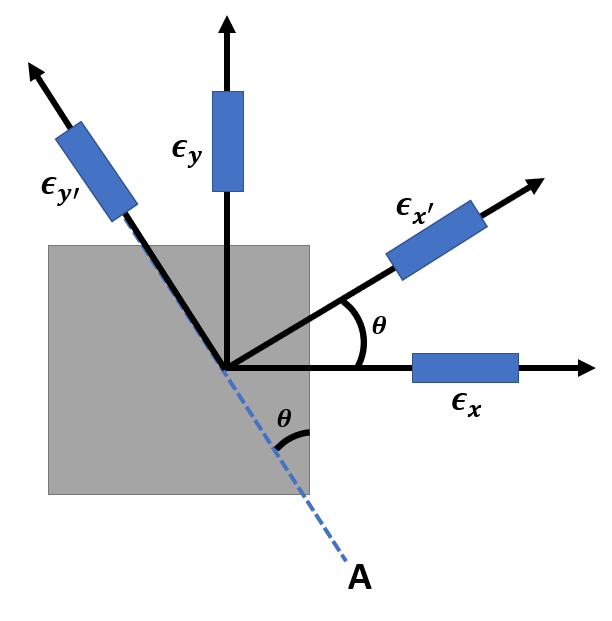
\includegraphics[scale=0.4]{rectangular_rosette.png}
				\end{figure}
			\end{itemize}\hrulefill
%-----------------------------------------------------------------------------------------%
	\subsection{Delta $\Delta$ rosette}
		\begin{itemize}
			\item If all the 3 gauges are at equal angular distance from one another, then its called \textbf{star rosette} or \textbf{delta rosette}
		\end{itemize}\hrulefill
%-----------------------------------------------------------------------------------------%
	\subsection{Star rosette}
		\begin{itemize}
			\item
		\end{itemize}\hrulefill
%-----------------------------------------------------------------------------------------%
	\section{Theories of Elastic failure}
		\begin{itemize}
			\item Generally there are two modes of failure:
				\begin{enumerate}
					\item Yielding or Ductile failure
					\item Fracture or Brittle failure
				\end{enumerate}
		\end{itemize}
		\subsection{Maximum Principal Stress theory - Rankine's Theory}
			\begin{itemize}
				\item Suitable for Brittle materials
				\item Material will fail if Max.Principal stress($\sigma_1$) = $\sigma_y$ in Tension
				\item Material will fail if Min.Principal stress($\sigma_3$) = $\sigma_y$ in Compression
				\item For no failure, $\sigma_1\le\sigma_y$ and For design, $\sigma_1\le\dfrac{\sigma_y}{FOS}$		
			\end{itemize}\hrulefill
%-----------------------------------------------------------------------------------------%
		\subsection{Maximum Principal strain theory - St.Venant's Theory}
			\begin{itemize}
				\item \textbf{Applicability and Limitations:}
				\item applicable for both ductile and brittle materials, but results are not accurate in both the cases
				\item In case of pure shear, results are still unsafe but better than Rankine's theory
				\item Material will fail if Max.Principal strain($\in_1$)=$\in_y$ under Uni-axial loading where $\boxed{\in_1=\dfrac{\sigma_1}{E}-\dfrac{\mu\sigma_2}{E}-\dfrac{\mu\sigma_3}{E}}$ and ${\in_y = \dfrac{\sigma_y}{E}}$
				\item For no failure, $\in_1\le\in_y$ and for design $\in_1\le\left(\dfrac{\sigma_P}{E}=\dfrac{\sigma_y}{FOS*E}\right)$
			\end{itemize}\hrulefill
%-----------------------------------------------------------------------------------------%
		\subsection{Maximum Shear stress theory - Guest \& Tresca's Theory}
			\begin{itemize}
				\item \textbf{Applicability and Limitations:}
				\begin{itemize}
					\item suitable for ductile materials and for pure shear case, it is over safe
					\item Not suitable for hydrostatic loading $\impliedby$ It says shear stress will be zero and so material will never fail, which not possible in reality.
					\item Not applicable to brittle materials as they have different yield stress in tension and compression
				\end{itemize}
				\item Material will fail when Max. Shear stress($\tau_{max}$) = $\dfrac{\sigma_y}{2}$ under uniaxial loading
				\item For no failure, $\tau_{max}\le\dfrac{\sigma_y}{2}$ and for design $\tau_{max}\le\dfrac{\sfrac{\sigma_y}{FOS}}{2}$
				\item Max shear stress in Bi-axial loading will be $\dfrac{\sigma_1-\sigma_2}{2}$
				\item Max shear stress in Tri-axial loading will be max$\left(\dfrac{\sigma_1-\sigma_2}{2},\dfrac{\sigma_2-\sigma_3}{2},\dfrac{\sigma_3-\sigma_1}{2}\right)$
			\end{itemize}\hrulefill
%-----------------------------------------------------------------------------------------%
		\subsection{Maximum Strain Energy theory - Haigh and Beltrami's Theory}
									
			\begin{itemize}
				\item \textbf{Applicability and Limitations:}
					\begin{itemize}
						\item suitable for ductile materials. Not suitable for brittle materials as elastic limit stress in tension and compression are quite different
						\item In case of pure shear, results are still unsafe for ductile materials
					\end{itemize}
				\item Material will fail when Max. Strain energy(u) = Strain energy developed at yield stress under Uni-axial loading $\implies \boxed{u = \dfrac{\sigma_y^2}{2E}}$
				\item for no failure, $u\le\dfrac{\sigma_y^2}{2E}$ and for design, $u\le\dfrac{\left(\sfrac{\sigma_y}{FOS}\right)^2}{2E}$
				\item $\boxed{u = \dfrac{1}{2E}(\sigma_1^2+\sigma_2^2-2\mu\sigma_1\sigma_2)} \impliedby$ (2D) $\;\;\;\boxed{u = \dfrac{1}{2E}\left[\sigma_1^2+\sigma_2^2+\sigma_3^2-2\mu(\sigma_1\sigma_2+\sigma_2\sigma_3+\sigma_3\sigma_1)\right]} \impliedby$ (3D)
			\end{itemize}\hrulefill
%-----------------------------------------------------------------------------------------%
		\subsection{Distortion energy theory - Mises-Henky Theory}
			\begin{itemize}
				\item \textbf{Applicability and Limitations:}
				\begin{itemize}
					\item suitable for ductile materials. For the case of pure shear, theoretical results is same as actual results
					\item Not applicable for brittle and not applicable under hydrostatic loading
				\end{itemize}
				\item Material will fail when $u_s=u_{ys} \impliedby$ Max.Shear strain energy = shear strain energy stored at yield stress in Uni-axial loading
				\item Total strain energy(u) = Volumetric strain energy($u_v$) + Shear strain energy($u_s$)
				\item $\boxed{u_v = \dfrac{1}{2}*\sigma_{avg}*\in_v}\;\;\;$ 
				\item $\boxed{\sigma_{avg} = \left(\dfrac{\sigma_1+\sigma_2+\sigma_3}{3}\right)}\;\;\;\boxed{u = \dfrac{1}{2E}\left[\sigma_1^2+\sigma_2^2+\sigma_3^2-2\mu(\sigma_1\sigma_2+\sigma_2\sigma_3+\sigma_3\sigma_1)\right]} \impliedby$ (3D)
				\item 
			\end{itemize}\hrulefill
%-----------------------------------------------------------------------------------------%
		\subsection{Octahedral Shear stress theory}
			\begin{itemize}
				\item
			\end{itemize}\hrulefill
%-----------------------------------------------------------------------------------------%
\end{document}
%-----------------------------------------------------------------------------------------%
%-----------------------------------------------------------------------------------------%
%-----------------------------------------------------------------------------------------%
